
\documentclass[main.tex]{subfiles}

\begin{document}

\part{傅里叶分析}
\setcounter{section}{0}

这一部分的符号有些混乱,请注意区分\(f(t), f[n], \hat{f}(\omega), \hat{f}(s), \hat{f}[z], \tilde{f}(t), \mathcal{F}[f(t)](\omega),\mathcal{F}[f[n]](\omega), \mathcal{F}[f[n]][k],\)
\newline
\( \mathcal{L}[f(t)](s), \mathcal{Z}[f(t)](z)\),接下来把这些符号梳理一遍.
\newline
\begin{itemize}
    \item[\(\bullet\)] \(f(t)\)表示一般的(时域上的)连续函数,该函数在整个\(\mathbb{R}\)上都有定义,自变量是\(t\),并赋予其时间的物理意义;
    \item[\(\bullet\)] \(f[n]\)表示一般的(时域上的)离散函数(即数列),该函数在整个\(\mathbb{Z}\)上都有定义,自变量使用\(n\)表示,并赋予其采样点序号的物理意义;
    \item[\(\bullet\)] \(\tilde{f}(\cdot)\)中的波浪上标可以加在任意一个域中的任意一个函数上,强调该函数是周期函数;
    \item[\(\bullet\)] \(\hat{f}(\cdot)\)中的尖角上标\(\hat{}\)表示该函数是变换域中的函数,自变量字母的选取表示该函数处在不同变换域;
    \item[\(\bullet\)] \(\mathcal{F}\left[f(t)\right](\omega)\),表示一个自变量是\(\omega\)的连续频域函数,由连续时域函数\(f(t)\)经过傅里叶变换得到,赋予\(\omega\)角频率的物理意义,赋予\(\xi=\dfrac{\omega}{2 \pi}\)频率的物理意义(字母\(f\)为函数专用,所以频率改用\(\xi\),这是傅里叶分析的书籍上惯用的字母). 
    \item[\(\bullet\)] \(\mathcal{F}\left[f[n]\right](\omega)\),表示一个自变量是\(\omega\)的连续频域函数,由离散序列\(f[n]\)经过离散时间傅里叶变换得到,赋予\(\omega\)角频率的物理意义.
    \item[\(\bullet\)] \(\mathcal{F}\left[f[n]\right][k]\),表示一个自变量是\(k\)的离散函数,由离散序列\(f[n]\)经过离散傅里叶变换得到,赋予\(k\)离散角频率的物理意义.
    \item[\(\bullet\)] \(\mathcal{L}\left[f(t)\right](s)\),表示一个自变量是\(s\)的连续函数,由连续函数\(f(t)\)经过双边拉普拉斯变换得到,赋予\(s\)复频率的物理意义.
    \item[\(\bullet\)] \(\mathcal{Z}\left[f[n]\right][z]\),表示一个自变量是\(z\)的离散函数,由离散序列\(f[n]\)经过双边Z变换得到,赋予\(z\)离散复频率的物理意义. 
\end{itemize}

注:以上这些变换本质上是函数到另一个函数的映射,凡是性质足够好的函数都可以应用这些变换,例如Schwartz空间及其对偶空间中的函数都可以进行傅里叶变换,变换后的函数仍属于该空间. 所以在此层面上并不存在所谓“时域”、“变换域”之类的说法,但为了贴合实际应用需要,我们往往通过其自变量使用的字母来区分这些域,同时也区分\(\mathcal{F}[\cdot]\)是哪一种傅里叶变换,例如我们认为\(f(t)=e^{-2t}\)是时域函数,\(\hat{f}(\omega)=e^{-2\omega}\)是连续频域内的函数,尽管这两个函数的对应法则是相同的,在\(\lambda\)演算层面都可以表示为\(\lambda x. e^{-2x}\).

\section{正交展开}

正交展开不是某种特殊的展开定理,而是一种重要的展开思想,首先回顾一下线性代数的知识.

\begin{reference}
    \(n\)维线性向量空间中只要确定了一组完备的基底\(\mathcal{A} = \{\bm{e}_1, \bm{e}_2, \cdots, \bm{e}_n\}\),则空间中的所有向量都可以用基底的线性组合表示出来:
    \[\bm{\alpha} = k_1\bm{e}_1+k_2\bm{e}_2+\cdots+k_n\bm{e}_n\]
    其中\(k_i\)是数,可以是实数、复数或其他无向的量.
    \newline
    如果空间中还定义了\textbf{内积},则称该向量空间为\textbf{内积空间},内积是一种运算,其结果为一个数量(实数或复数),两个向量的内积记为\(\langle \bm{\alpha},\bm{\beta} \rangle\),满足
    \begin{itemize}
        \item [(1)] \(\langle \bm{\alpha},\bm{\beta} \rangle = \overline{\langle \bm{\beta},\bm{\alpha} \rangle}\),上划线表示取共轭,如果内积运算定义在实数域上,则有\(\langle \bm{\alpha},\bm{\beta} \rangle = \langle \bm{\beta},\bm{\alpha} \rangle\).
        \item [(2)] \(\langle m\bm{\alpha}+n\bm{\beta},\bm{\gamma} \rangle = m\langle \bm{\alpha},\bm{\gamma} \rangle + n\langle \bm{\beta},\bm{\gamma} \rangle\),其中\(m,n\)是数量.
        \item [(3)] \(\langle \bm{\alpha},\bm{\alpha} \rangle \geq 0\),当且仅当\(\bm{\alpha}=\bm{0}\)时等号成立.
    \end{itemize}
    定义了内积之后,向量的\textbf{模长}便可定义为\(\|\bm{\alpha}\|=\sqrt{\langle \bm{\alpha},\bm{\alpha} \rangle}\),易知\(\|\bm{\alpha}\| \geq 0\);
    \newline
    线性组合的系数可表示为\(k_i=\dfrac{\langle \bm{\alpha}, \bm{e}_i \rangle}{\langle \bm{e}_i, \bm{e_i} \rangle}\),成为向量\(\bm{\alpha}\)在向量\(\bm{e}_i\)上的\textbf{投影}.
    \newline
    向量的\textbf{正交}则表示\(\langle \bm{\alpha},\bm{\beta} \rangle=0\)这种情况,可简记为\(\bm{\alpha} \perp \bm{\beta}\).
    \newline
    假设\(\mathcal{A}=\{\bm{e}_1, \bm{e}_2, \cdots, \bm{e}_n\}\)是自然基,即两两正交且\(\|\bm{e}_i\|=1\),则立即可以确定线性组合的系数:\(k_i = \langle\bm{\alpha},\bm{e}_i\rangle\),而模也可以立即确定为\(\|\bm{\alpha}\| = \sqrt{k_1^2+k_2^2+\cdots+k_n^2} = \sqrt{\langle\bm{\alpha},\bm{e}_1\rangle^2+\langle\bm{\alpha},\bm{e}_2\rangle^2+\cdots+\langle\bm{\alpha},\bm{e}_n\rangle^2}\)
\end{reference}

正交展开的核心就是这些,但以上只给了抽象的框架,具体操作起来大有可为. 

仔细思考线性组合的式子:\(\bm{\alpha} = k_1\bm{e}_1+k_2\bm{e}_2+\cdots+k_n\bm{e}_n\),它想表达的是\(\bm{\alpha}\)可以由向量\(e_1, e_2, \cdots, e_n\)各自贡献一点组合而成,投影即系数\(k_i\)定量描述了向量\(\bm{e}_i\)贡献的大小. 如果为\(k_i=0\)表示向量\(\bm{e}_i\)没有贡献,此时得到的\(\bm{\alpha}\)和\(\bm{e_i}\)无关,或称正交.

在函数空间中,函数就是向量,它的内积有一套独特的定义,但大多数教材并没有解释为什么要这么定义,以下是一种可能的理解.

\textit{
线性代数告诉我们,实区间\([a,b]\)上的连续实变函数构成了一个线性空间,但函数空间不像向量空间那么直观,它的内积并没有那么容易定义出来。假设函数\(f\)在实区间\([a,b]\)上等距抽样,例如间隔\(\dfrac{1}{n}\)取值,然后用一个向量\(\vec{\bm{u}}_f\)来记录这些值:
\[\vec{\bm{u}}_f = \left[f(a), f(a+\frac{b-a}{n}), f(a+\frac{2(b-a)}{n}), f(a+\frac{3(b-a)}{n}), \cdots, f(a+\frac{(n-1)(b-a)}{n}), f(b)\right]\]
对于另一个在区间\([a,b]\)上连续的函数\(g(x)\),也采用相同的操作:
\[\vec{\bm{u}}_g = \left[g(a), g(a+\frac{b-a}{n}), g(a+\frac{2(b-a)}{n}), g(a+\frac{3(b-a)}{n}), \cdots, g(a+\frac{(n-1)(b-a)}{n}), g(b)\right]\]
此时对两个向量求内积:
\[\langle\vec{\bm{u}}_f,\vec{\bm{u}}_g\rangle = f(a)g(a)+f(a+\frac{b-a}{n})g(a+\frac{b-a}{n})+f(a+\frac{2(b-a)}{n})g(a+\frac{2(b-a)}{n})+\cdots+f(b)g(b)\]
现在令\(n \to \infty\),意味着抽样间隔\(\dfrac{1}{n} \to 0\),由于两个函数都是连续函数,不会发生跳跃,因此可以认为\(\vec{\bm{u}}_f\)和\(\vec{\bm{u}}_g\)这两个向量记录了函数的所有信息. 但是这样的内积往往会趋近于无穷大. 由于是等距抽样,每个样本的权重相等,所以在每个单项式上乘以权重\(1/n\),然后奇迹般地凑出了积分的定义式
\[\lim_{n \to \infty}\frac{1}{n}\langle\vec{\bm{u}}_f,\vec{\bm{u}}_g\rangle = \lim_{n \to \infty}\frac{1}{n}\sum_{k=0}^{n}f(a+\frac{k(b-a)}{n})g(a+\frac{k(b-a)}{n}) := \int_{a}^{b} f(x)g(x)\trm{d}x\]
以上是实变函数的情况,在这种情况下,才满足\([f(x)]^2\equiv|f(x)|^2\),根据定积分的保号性,这即可满足线性空间中\(\|f\|\geq 0\)的要求. 如果扩展到复变函数,由于两个复数的乘积还是复数,复变函数作定积分以后也是复数,不一定能与\(0\)比大小,所以为了符合模长的定义,需要将被积函数由\([f(z)]^2\)改为\(|f(z)|^2\),而后者等价于\(f(z)\overline{f(z)}\),这就得到了复变函数空间的内积.
}
\begin{definition}{函数空间的内积}
    对于在复连通域\(D\)上定义的连续函数\(f(z),g(z)\),规定其\uline{内积}(inner product)为
    \[ \langle f,g \rangle := \int_{D} f(z)\overline{g(z)}\trm{d}z\]
    若\(\langle f,g \rangle=0\),则称这两个函数是\uline{正交的}(orthonormal). 函数的模定义为
    \[ \|f\| := \sqrt{\int_{D}f(z)\overline{f(z)}\trm{d}z}\]
    当复连通域定退化为区间\([a,b]\)时,复变函数退化为实变函数时,其内积便退化为
    \[ \langle f,g \rangle := \int_{a}^{b} f(x)g(x)\trm{d}x\]
    模长退化为
    \[ \|f\| := \sqrt{\int_{a}^{b}[f(x)]^2\trm{d}x}\]
\end{definition}

定义好函数空间的内积之后,便可以尝试在空间中寻找一组函数作为基底\(\mathcal{A}=\{\varphi_1,\varphi_2,\varphi_3,\cdots\}\),然后把空间中的任意都写成它们的线性组合的形式,
\[f(z) = c_1\varphi_1(z)+c_2\varphi_2(z)+c_3\varphi_3(z)+\cdots\]
如果基底\(\mathcal{A}\)是正交基底,则可以进一步得到
\[c_n=\frac{\langle f,\varphi_n \rangle}{\langle \varphi_n,\varphi_n \rangle} = \frac{\langle f,\varphi_n \rangle}{\|\varphi_n\|^2} = \frac{\displaystyle{\int_{D} f(z)\overline{\varphi_n(z)}\trm{d}z}}{\displaystyle{\int_{D}\varphi_n(z)\overline{\varphi_n(z)}\trm{d}z}}\]
这便是正交展开的基本思路,由于这个思路最早应用在傅里叶级数上,所以又称这种展开方式为\uline{广义傅里叶展开}.

\textit{
    以上有个细节需要注意,函数空间的基底写成\(\mathcal{A}=\{\varphi_1,\varphi_2,\varphi_3,\cdots\}\)而不是\(\mathcal{A}=\{\varphi_1,\varphi_2,\varphi_3,\cdots,\varphi_n\}\),是因为基向量的个数可能是无限的,甚至可能是不可数无穷多的. 如果是实数多个的基向量\(\mathcal{A}=\{\varphi_s\}_{s \in I}\),那么每个基向量的分量\(c_s\)中的下标取值也不再可数,此时\(f(z)\)就不能简单地展开成基向量线性组合的形式,而是像上面那样间隔取样,缩小间隔,最后凑出积分的形式,即
    \[f(z)=\int_{I}c_s\varphi_s(z)\trm{d}s\]
    剧透一下,这实际上就是傅里叶反变换公式的意义.
}

最后简单总结一下什么是正交展开. 如果向量\(\bm{\alpha}\)属于线性空间\(S\),那么总是可以找到一组完备的正交基\footnote{“所有线性空间,无论维数有穷还是无穷,都能找到一组完备的正交基底”这个命题依赖于选择公理},使得\(\bm{\alpha}\)可以被这组基底线性表出,该线性表出式就是向量\(\bm{\alpha}\)的正交展开.

\section{平行地导出傅里叶级数和傅里叶变换}

有了正交展开的思想,我们就可以摧枯拉朽般的导出傅里叶级数和连续傅里叶变换,流畅自然的程度令带积分余项的泰勒公式也自愧不如,而不用像很多教材那样再拿三角函数的积分倒来倒去,这也是连续傅里叶变换和傅里叶级数能写在一起的原因.
\vspace{1cm}
\newline
\noindent \textbf{
\(\bullet\)导出\([t_0, t_0+T]\)上三角函数形式的傅里叶级数:基底\(\mathcal{A}=\{\sin(n\omega t), \cos(n\omega t)\}_{n=0}^{\infty}\)(\(\sin(0\omega t)\)除外)
}

需要注意,这里的\(\omega=\dfrac{2\pi}{T}\),有角频率的物理意义,这也限定了\(\sin(n\omega t)\)和\(、cos(n\omega t)\)的周期都是\(T\)。首先验证这些基底确实是正交的,别忘了三个积化和差公式,这里贴心地把它们写出来:
\begin{align*}
    \sin\alpha\cos\beta &= +\frac{1}{2}\left[\sin(\alpha+\beta)+\sin(\alpha-\beta)\right] \\
    \sin\alpha\sin\beta &= -\frac{1}{2}\left[\cos(\alpha+\beta)-\cos(\alpha-\beta)\right] \\
    \cos\alpha\cos\beta &= +\frac{1}{2}\left[\cos(\alpha+\beta)+\cos(\alpha-\beta)\right]
\end{align*}
带入计算内积:
\begin{align*}
    \forall m,n\in \mathbb{N},\quad m \neq n: & \\
    \langle \sin(m\omega t), \cos(n\omega t) \rangle &:= \int_{t_0}^{t_0+T} \sin(m\omega t)\cos(n\omega t) \trm{d}t = -\left[\frac{\cos((m-n)\omega t)}{2(m-n)\omega}+\frac{\cos((m+n)\omega t)}{2(m+n)\omega}\right]_{t_0}^{t_0+T} = 0 \\
    \langle \sin(m\omega t), \sin(n\omega t) \rangle &:= \int_{t_0}^{t_0+T} \sin(m\omega t)\sin(n\omega t) \trm{d}t = \left[\frac{\sin((m-n)\omega t)}{2(m-n)\omega}-\frac{\sin((m+n)\omega t)}{2(m+n)\omega}\right]_{t_0}^{t_0+T} = 0 \\
    \langle \cos(m\omega t), \cos(n\omega t) \rangle &:= \int_{t_0}^{t_0+T} \cos(m\omega t)\cos(n\omega t) \trm{d}t = \left[\frac{\sin((m-n)\omega t)}{2(m-n)\omega}+\frac{\sin((m+n)\omega t)}{2(m+n)\omega}\right]_{t_0}^{t_0+T} = 0
\end{align*}
内积都是0,所以正交. 接下来求出它们的模长:
\begin{align*}
    \|1\| &= \sqrt{\int_{t_0}^{t_0+T}\trm{d}t} = \sqrt{T} \\
    \|\cos(n\omega t)\| &= \sqrt{\int_{t_0}^{t_0+T} \cos^2(n\omega t) \trm{d}t} = \sqrt{\frac{T}{2}},\quad n \in \mathbb{N}^* \\
    \|\sin(n\omega t)\| &= \sqrt{\int_{t_0}^{t_0+T} \sin^2(n\omega t) \trm{d}t} = \sqrt{\frac{T}{2}},\quad n \in \mathbb{N}^*
\end{align*}
这时候满足某些条件的函数就可以做正交展开:
\[f(t) = \frac{\langle f(t), 1 \rangle}{\|1\|^2} + \sum_{n=1}^{\infty} \left[\frac{\langle f(t), \sin(n\omega t) \rangle}{\|\sin(n\omega t)\|^2}\sin(n\omega t) + \frac{\langle f(t), \cos(n\omega t) \rangle}{\|\cos(n\omega t)\|^2}\cos(n\omega t)\right]\]
这就是周期为\(T\)的傅里叶级数,整理一下就好.

\begin{definition}{三角函数形式的傅里叶级数}
    定义在区间\([t_0,t_0+T]\)上的函数\(f(t)\),将
    \[S_{\infty}[f](t) = \frac{a_0}{2}+\sum_{n=1}^{\infty} \left[a_n\cos(n\omega t)+b_n\sin(n\omega t)\right]\]
    称为\(f(t)\)的三角函数形式的\uline{傅里叶级数}(Fourier series),其中
    \begin{align*}
        a_n &= \frac{2}{T}\int_{t_0}^{t_0+T} f(t)\cos(n\omega t)\trm{d}t \\
        b_n &= \frac{2}{T}\int_{t_0}^{t_0+T} f(t)\sin(n\omega t)\trm{d}t \\
        \omega &= \frac{2\pi}{T}
    \end{align*}
\end{definition}

嘿!上面已经说好了\(f(t)\)等于这一大串级数,为什么这里又要搞出个\(S_{\infty}[f](t)\)出来呢?先卖个关子,等讨论到收敛性的时候就会发现\(f(t)\)需要满足一定的条件才能让\(S_{\infty}[f](t)\)收敛到\(f(t)\)上,而且收敛的方式也值得探究.

\vspace{1cm}
\noindent \textbf{
\(\bullet\)导出\([t_0, t_0+T]\)上极坐标形式的傅里叶级数:基底\(\mathcal{A}=\{A_n\sin(n\omega t+\varphi_n)\}_{n=0}^{\infty}\)
}

你以为我又会验证一遍正交性,再计算模长,然后还要求出每个\(A_n\)和\(\varphi_n\)的表达式?辅助角公式它不香吗?
\[A\sin(t)+B\cos(t)=\sqrt{A^2+B^2}\sin(t+\arctan\frac{B}{A}) = \sqrt{A^2+B^2}\cos(t+\trm{arccot}\frac{B}{A})\]
把正弦项和余弦项合并,就得到了
\begin{definition}{极坐标形式的傅里叶级数}
    定义在区间\([t_0,t_0+T]\)上的函数\(f(t)\),将
    \[S_{\infty}[f](t) = \frac{a_0}{2}+\sum_{k=1}^{\infty} A_k{\color{red}\sin}(k\omega t+\varphi_k) = \frac{a_0}{2}+\sum_{k=1}^{\infty} A_k{\color{red}\cos}(k\omega t+\psi_k)\]
    称为\(f(t)\)的极坐标形式的傅里叶级数,其中
    \[
        \begin{aligned}
            & A_k = \sqrt{a_k^2+b_k^2},  && \omega = \frac{2\pi}{T} \\
            & \varphi_k = \arctan\frac{b_k}{a_k}, && \psi_k = \trm{arccot}\frac{b_k}{a_k}
        \end{aligned}
    \]
\end{definition}

极坐标形式的傅里叶级数用得最少,但它证实了傅里叶的大胆猜测:每一个周期函数都可以表示为多个正弦函数的叠加. 此时的参数\(A_k\)和\(\varphi_k\)就具有了物理意义,前者表示振幅,后者表示初相;而最前面的\(a_0/2\)就表示一个周期内函数的均值,用来修正上下平移.

\vspace{1cm}
\noindent \textbf{
\(\bullet\)导出\([t_0, t_0+T]\)上复数形式的傅里叶级数:基底\(\mathcal{A}=\{e^{in\omega t}\}_{n=-\infty}^{\infty}\)
}

根据欧拉公式替换三角函数:
\[ \cos(t) = \frac{e^{it}+e^{-it}}{2}, \qquad \sin(t) = -i\frac{e^{it}-e^{-it}}{2} \]
然后整理三角函数项的傅里叶级数表达式
\begin{align*}
    S_{\infty}[f](t) &= \frac{a_0}{2}+\sum_{k=1}^{\infty} \left[a_k\sin(k\omega t)+b_k\sin(k\omega t)\right] \\
    &= \frac{a_0}{2} + \sum_{k=0}^{\infty}\left(a_k\frac{e^{ik\omega t}+e^{-ik\omega t}}{2}-ib_k\frac{e^{ik\omega t}-e^{ik\omega t}}{2} \right) \\
    &= \frac{a_0}{2}+\sum_{k=1}^{\infty}\left( \frac{a_k-ib_k}{2}e^{ik\omega t}+\frac{a_k+ib_k}{2}e^{-ik\omega t}\right)
\end{align*}
其中
\[\frac{a_k \pm ib_k}{2} = \frac{1}{T}\int_{t_0}^{t_0+T}f(t)\left[\cos(k\omega t) \pm i\sin(k\omega t) \right] \trm{d}t = \frac{1}{T}\int_{t_0}^{t_0+T}f(t)e^{\pm ik\omega t}\trm{d}t\]
回代,得到
\[f(t) = \frac{a_0}{2} + \sum_{k=0}^{\infty}\left[ \frac{1}{T} \int_{t_0}^{t_0+T}f(t)e^{-ik\omega t}\trm{d}te^{ik\omega t}+ \frac{1}{T}\int_{t_0}^{t_0+T}f(t)e^{ik\omega t}\trm{d}te^{-ik\omega t}\right]\]
若令\(\displaystyle{c_k = \frac{1}{T} \int_{t_0}^{t_0+T}f(t)e^{-ik\omega t}\trm{d}t}\),则易验证\(\displaystyle{\frac{a_0}{2} = c_0}\),此时就有
\begin{definition}{复数项形式的傅里叶级数}
    定义在区间\([t_0,t_0+T]\)上的函数\(f(t)\),将
    \[S_{\infty}[f](t) = \sum_{k=-\infty}^{+\infty}c_ke^{ik\omega t}\]
    称为\(f(t)\)的复数项形式的傅里叶级数,其中
    \[c_k = \frac{1}{T} \int_{t_0}^{t_0+T}f(t)e^{-ik\omega t}\trm{d}t, \qquad \omega=\frac{2\pi}{T}\]
\end{definition}

复数项的傅里叶级数,看起来比三角函数项的傅里叶级数简洁. 由推导公式可以看出,复数项级数的系数\(c_k=\dfrac{a_k-ib_k}{2}\),反过来有\(a_k=2\trm{Re}[c_k], \,\, b_k=-2\trm{Im}[c_k]\).

\vspace{1cm}
\noindent \textbf{
\(\bullet\)导出连续傅里叶级数:基底\(\mathcal{A}=\{e^{i\omega t}\}_{\omega \in \mathbb{R}}\)
}

由于基底有不可数无穷多个,所以应该把求和换成积分;由于基底是复变函数,所以作内积的时候记得取共轭,即原函数在基底\(e^{i\omega t}\)上的投影:
\[c_\omega = \langle f(t), e^{i\omega t} \rangle = \int_{\mathbb{R}}f(t)e^{-i\omega t}\trm{d}t\]
而原函数:
\[f(t) = \int_{\mathbb{R}}c_\omega e^{i\omega t}\trm{d}\omega\]
这其实就是连续傅里叶变换.

\begin{definition}{傅里叶变换}
    对于函数\(f(t)\),
    \[\hat{f}(\omega) = \mathcal{F}[f(t)](\omega) := \int_{-\infty}^{\infty}f(t)e^{-i\omega t}\trm{d}t\]
    如果存在,则称为\(f(t)\)的\uline{傅里叶变换}(Fourier transform),其反变换为
    \[f(t) = \mathcal{F}^{-1}[\hat{f}(\omega)](t) := \frac{1}{2\pi}\int_{-\infty}^{\infty}\hat{f}(\omega)e^{i\omega t}\trm{d}\omega\]
    \(f(t)\)的定义域一般称为\uline{时域}(time domain),\(\hat{f}(\omega)\)的定义域一般称为\uline{频域}(frequency domain).
\end{definition}

太快啦,一下子推出了三种傅里叶级数,现在把脚步放慢,
这里,我们需要验证一下基底的正交性,计算基底的模长.

% 可以对比一下复数项的傅里叶级数和洛朗级数(\(z=0\)处展开):
% \[
% \begin{aligned} 
%     & \mbot{洛朗级数:} & f(t) &= \sum_{n=-\infty}^{\infty} a_nt^n, && a_n = \frac{f^{(n)}(0)}{n!} \\
%     & \mbot{复数项的傅里叶级数:}  & f(t) &= \sum_{n=-\infty}^{\infty} c_ne^{in\omega t}, && c_n = \int_T f(t)e^{-ik\omega t}\trm{d}t
% \end{aligned}
% \]
% 这两者看起来毫无关系,...

\vspace{1cm}

\subsubsection{傅里叶级数作为原函数的延拓}

以上导出傅里叶级数的时候,特别强调了区间是\([t_0,t_0+T]\),尽管在本章最开始时规定了\(f(t)\)必须在整个\(\mathbb{R}\)上有定义,但回顾刚才导出的过程,\(f(t)\)即使在该区间以外没有定义也不影响该区间内傅里叶级数的存在. 与此同时,\(S_{\infty}[f](t)\)作为一系列三角函数的和,在区间外仍然有定义,并且考虑到这些三角函数的角频率是\(\omega, 2\omega, 3\omega, \cdots\)、最小正周期是\(T, T/2, T/3, \cdots\),因此\(T\)是\(S_{\infty}[f](t)\)是的最小正周期. 这意味着\(S_{\infty}[f](t)\)会在整个\(\mathbb{R}\)上不断重复着\([t_0,t_0+T]\)的故事,这就把一个可能只在原区间内连续的函数\(f(t)\)伸展成了在\(\mathbb{R}\)上定义的、以\(T\)为周期的函数\(S(t)\),即称为\uline{延拓}(continuation).

若\(f(t)\)是奇函数或偶函数,那么其定义区间关于原点对称,此时\(\{a_n\}\)和\(\{b_n\}\)有一串全是\(0\),此时傅里叶级数只剩下正弦(奇函数)或余弦项(偶函数),此时就称其为\uline{正弦级数}或\uline{余弦级数}. 

如果被展开的函数\(f(t)\)只在区间\([0,T]\)上有定义,用傅里叶级数可以给予其两种不同的延拓,一种是\uline{奇延拓},即构造奇函数\(g(t)\)
\[g(t)=\begin{cases} f(t) \qquad t\in[0,T] \\ -f(-t) \qquad t \in [-T,0]\end{cases}\]
另一种延拓方式是\uline{偶延拓}
\[g(t)=\begin{cases} f(t) \qquad t\in[0,T] \\ -f(-t) \qquad t \in [-T,0]\end{cases}\]
然后对\(g(t)\)进行傅里叶展开,就可以得到正弦级数和余弦级数.

以下是一些常用周期函数的傅里叶展开
\newline
(1) 梯形波(奇函数)
\[f(t)\sim\frac{4A}{\pi\omega d}\sum_{n\,\trm{odd}}\sin\left(\frac{n\omega d}{n^2}\right)\sin(n\omega t)\]
(2) 矩形脉冲(偶函数)
\[f(t)\sim\alpha A + \frac{2A}{\pi}\sum_{n=1}^{\infty}\frac{\sin(\alpha n \pi)}{n} \cos(n\omega t)\]
(3) 方波(奇函数)
\[f(t) \sim \frac{4A}{\pi}\sum_{n\,\trm{odd}} \frac{\sin(n\omega t)}{n}\]
(4) 三角波(奇函数)
\[f(t) \sim \frac{8A}{\pi^2}\sum_{n\,\trm{odd}}\frac{i^{n-1}\sin(n\omega t)}{n^2}\]
(5) 锯齿波(非奇非偶)
\[f(t) \sim \frac{A}{2}-\frac{A}{\pi}\sum_{n=1}^{\infty} \frac{\sin(n\omega t)}{n}\]


\subsection{傅里叶级和傅里叶变换的联系}

刚才平行地导出了傅里叶级数和傅里叶变换,很快也很自然,但傅里叶级数和傅里叶变换的联系却被忽略了,这一节就来补上这部分的内容。

联系向量相加的几何意义,向量的基分解公式告诉我们,空间中任意一个向量\(\vec{\alpha}\)都可以由每一个\(\vec{\varepsilon}_n\)伸长或缩短为为原来的\(a_n\)倍之后首尾相接得到. 由于\(e^{in\omega t}\)在复平面上表现为一个以角速度\(n\omega\)旋转的单位向量. 所以复数项的傅里叶级数告诉我们,\(f(t)\)(更准确地说是起点位于原点、终点在实轴上\(f(t)\)处的向量)可以由多个正在分别以角速度\(\{\cdots, -2\omega, -\omega, 0, \omega, 2\omega, \cdots\}\)旋转、长度分别为\(\{\cdots, c_{-2}, c_{-1}, c_0, c_1, c_2, \cdots\}\)的向量首尾相接得来(负的角速度表示方向相反),同时还能保证这些向量首尾相接之后终点恰好在实轴上.

然而这些旋转向量的角速度是分立的,存在角速度为\(\omega\)的旋转向量,也存在角速度为\(\omega\)的旋转向量,却不存在角速度为\(1.5\omega\)的旋转向量. 角速度值最小间隔是\(\Delta \omega = \omega =\dfrac{2\pi}{T}\). 如果将\(T\)增大,那么\(\Delta \omega\)就会减小,当\(T\to\infty\)时,\(\Delta \omega \to 0\),这时可以认为\(f(t)\)展开的基底是\(\mathcal{A}=\{e^{i\omega t}\}_{\omega \in \mathbb{R}}\),根据正交展开的思想,这时应该改写为
\[f(t)=\int_{\mathbb{R}}c_\omega e^{i\omega t}\trm{d}t\]
其中系数
\[c_\omega = \frac{\langle f(t), e^{i\omega t} \rangle}{\langle e^{i\omega t},e^{i \omega t} \rangle} = \int_{\mathbb{R}}f(t)\overline{e^{i\omega t}}\trm{d}t=\int_{\mathbb{R}}f(t)e^{-i\omega t}\trm{d}t\]
这就是傅里叶变换及其反变换,但你会发现\(\langle e^{i\omega t},e^{i \omega t} \rangle\)似乎算不出来,所以为了严谨起见,以下仍通过定积分导出. 关于这个内积到底怎么算,接下来会通过严格定义某些东西把它彻底解决.


\vspace{0.5cm}

设\(\Delta\omega=\Omega_n-\Omega_{n-1}=\dfrac{2\pi}{T}\),把区间移回\([-\dfrac{T}{2},\dfrac{T}{2}]\),然后复数项的傅里叶级数就可以写为
\begin{align*}
    f(t) &= \lim_{T \to \infty}\sum_{k=-\infty}^{+\infty}c_ke^{-ik\omega t} \\
    &= \lim_{T \to \infty}\sum_{k=-\infty}^{+\infty}\frac{1}{T} \int_{-\frac{T}{2}}^{\frac{T}{2}}f(t)e^{-ik\omega t}\trm{d}t\cdot e^{ik\omega t} \\
    &= \lim_{\Delta\omega \to 0}\sum_{k=-\infty}^{+\infty} \left[\int_{-\frac{\pi}{\Delta\omega}}^{\frac{\pi}{\Delta\omega}}f(t)e^{-ik\omega t}\trm{d}t \right]e^{ik\omega t}\frac{\Delta\omega}{2\pi}
\end{align*}
这个式子很长,但这恰好是定积分的定义,最终得到
\[ f(t) = \frac{1}{2\pi}\int_{-\infty}^{\infty} \left[\int_{-\infty}^{\infty}f(t)e^{-i\omega t}\trm{d}t \right]e^{i\omega t}\trm{d}\omega \]
称为\uline{傅里叶积分公式}. 现在可以给出定义了.

\begin{definition}{傅里叶变换}
    对于函数\(f(t)\),
    \[\hat{f}(\omega) = \mathcal{F}[f(t)](\omega) := \int_{-\infty}^{\infty}f(t)e^{-i\omega t}\trm{d}t\]
    如果存在,则称为\(f(x)\)的\uline{傅里叶变换}(Fourier transform),其中\(\mathcal{F}\)表示傅里叶变换算子,其反变换为
    \[f(t) = \mathcal{F}^{-1}[\hat{f}(\omega)](t) := \frac{1}{2\pi}\int_{-\infty}^{\infty}\hat{f}(\omega)e^{i\omega t}\trm{d}\omega\]
    \(f(t)\)的定义域一般称为\uline{时域}(time domain),\(\hat{f}(\omega)\)的定义域一般称为\uline{频域}(frequency domain).
\end{definition}
\(\mathcal{F}\)是一个定义在函数空间上的函数,即所谓的“函数的函数”,用类型论的语言来表示,由于\(f:\mathbb{R}\to\mathbb{R}\),\(\hat{f}:\mathbb{R}\to\mathbb{R}\),所以\(\mathcal{F}:(\mathbb{R}\to\mathbb{R})\to(\mathbb{R}\to\mathbb{R})\). 

\vspace{1cm}

仔细思考傅里叶变换的意义,为什么称\(\hat{f}(\omega)\)的定义域为“频域”呢?回到复数项形式的傅里叶级数:
\[f(x) = \sum_{n=-\infty}^{\infty}c_ne^{in\omega x}\]


以上表明复数项的傅里叶级数的本质是函数在正交基底上的分解公式,那么傅里叶变换呢?在单位正交基底中,某个向量\(\vec{\alpha}\)在某个基底向量上\(\vec{\varepsilon}_n\)的投影为\(\vec{\alpha}_n = \langle \vec{\alpha},\vec{\varepsilon}_n \rangle\). 代入函数空间\(\mathbb{R}\)中两个函数的内积定义(至于为什么这样定义,参见3.1节),函数\(f(t)\)在函数\(\psi_{\xi}(t)\)上的投影:
\[f(\xi) = \langle f(t), \psi_{\xi}(t) \rangle = \int_{-\infty}^{\infty}f(t)\psi_{\xi}(t)\trm{d}t\]
同时看一看傅里叶变换的定义:
\[\hat{f}(\omega) = \int_{-\infty}^{\infty}f(t)e^{-i\omega t}\trm{d}t\]
两个公式的结构很相似,只要定义\(\psi_{\xi}(t)=e^{-i\xi t}\)就在形式上完全相同了,不过想把两者真正联系起来,还有两点需要补充.
\begin{itemize}
    \item [\(\bullet\)] \(\psi_{\xi}(t)=e^{-i\xi t}\)是单位向量,即模长为1. 
    \newline
    \textit{
        证明:这是显然的.
    }
    \item [\(\bullet\)] 当参数\(\xi\neq\rho\)时,函数\(\psi_{\xi}(t)\)和\(\psi_{\rho}(t)\)是正交的. 
    \newline
    \textit{
        证明:证明\(\psi_{\xi}(t)\)和\(\psi_{\rho}(t)\)内积为\(0\)即可.
        \[\langle \psi_{\xi}(t),\psi_{\rho}(t) \rangle = \int_{-\infty}^{\infty}\overline{\psi_{\xi}(t)}\psi_{\rho}(t)\trm{d}t = \int_{-\infty}^{\infty}e^{-i(\xi-\rho)t}\trm{d}t\]
        下一节会提到这个积分实际上等效于\(\delta\)函数.
        \[\langle \psi_{\xi}(t),\psi_{\rho}(t) \rangle \sim 2\pi\delta(\xi-\rho)\]
        因此只要\(\rho \neq \xi\)内积就可认为是\(0\).
    }
\end{itemize}

联系概率论的知识,当随机变量的取值变的稠密甚至连续的时候,就不适合用概率函数\(P(X)\)而应该用概率密度函数\(p(x)\)了,此处的思想也相同,当频率可取的值连续的时候,\(\hat{f}(\omega)\)表示的是频率的“密度”.

\subsubsection{傅里叶变换的性质}

傅里叶变换有以下性质(记\(\hat{f}(\omega)=\mathcal{F}[f(t)](\omega)\)):\\

\begin{itemize}
    \item [(1)] 线性
    \[ \mathcal{F}\left[a_1f_1(t)+a_2f_2(t)\right](\omega) = a_1\hat{f}_1(\omega)+a_2\hat{f}_2(\omega)\]
    \textit{
        证明:直接套定义,利用积分的线性性质
    }
    \begin{align*} 
        \mathcal{F}\left[a_1f_1(t)+a_2f_2(t)\right](\omega) &= \int_{\infty}^{\infty}\left[a_1f_1(t)+a_2f_2(t)\right]e^{-i\omega t}\trm{d}t \\
        &= a_1\int_{\infty}^{\infty}f_1(t)e^{-i\omega t}\trm{d}t + a_2\int_{\infty}^{\infty}f_2(t)e^{-i\omega t}\trm{d}t \\
        &= a_1\hat{f}_1(\omega)+a_2\hat{f}_2(\omega)
    \end{align*}
    \item [(2)] 共轭对称性
    \[ \mathcal{F}\left[\overline{f(t)}\right](\omega) = \overline{\hat{f}(-\omega)}\]
    \textit{
        证明:由于\(f(t)=|f(t)|\exp(i\trm{Arg}[f(t)])\),所以
    }
    \[\mathcal{F}\left[\overline{f(t)}\right](\omega) = \int_{-\infty}^{\infty}|f(t)|e^{-i\trm{Arg}[f(t)]}e^{-i\omega t}\trm{d}t = \int_{-\infty}^{\infty}\overline{|f(t)|e^{i\trm{Arg}[f(t)]}e^{i\omega t}}\trm{d}t = \overline{\hat{f}(-\omega)}\]
    \item [(3)] 时域-频域对偶
    \[ \mathcal{F}\left[\hat{f}(\omega)\right](t) = 2\pi f(-t)\]
    \textit{
        证明:直接套定义
    }
    \[\mathcal{F}\left[\hat{f}(t)\right](\omega) = \int_{-\infty}^{\infty}\hat{f}(t)e^{i(-\omega)t}\trm{d}t = 2\pi\mathcal{F}^{-1}\left[\hat{f}(t)\right](-\omega) = 2\pi f(-\omega)\]
    \item [(4)] 平移
    \begin{align*} 
        \mathcal{F}\left[f(t-t_0)\right](\omega) &= \hat{f}(\omega)e^{-i\omega t_0} \\
        \mathcal{F}\left[\hat{f}(\omega-\omega_0)\right](t) &= 2\pi f(t)e^{-i\omega_0t}
    \end{align*}
    \textit{
        证明:还是直接套定义
    }
    \[ \mathcal{F}\left[f(t-t_0)\right](\omega) = \int_{-\infty}^{\infty} f(t-t_0)e^{-i\omega t}\trm{d}t\]
    \textit{令\(\tau = t-t_0\),得}
    \[ \mathcal{F}\left[f(t-t_0)\right](\omega) = \int_{-\infty}^{\infty} f(\tau)e^{-i\omega(\tau+t_0)}\trm{d}t = e^{-i\omega t_0}\int_{-\infty}^{\infty} f(\tau)e^{-i\omega(\tau)}\trm{d}t = e^{-i\omega t_0}\hat{f}(\omega) \]
    \item [(5)] 缩放
    \[ \mathcal{F}\left[f(at)\right](\omega) = \frac{1}{|a|}\hat{f}\left(\frac{\omega}{a}\right) \]
    \item [(6)] 全域积分值
    \[ \int_{-\infty}^{+\infty}f(t)\trm{d}t = \hat{f}(0)\]
    \[ \int_{-\infty}^{+\infty}\hat{f}(\omega)\trm{d}\omega = 2\pi f(0)\]
    \textit{证明:在定义式中令\(\omega=0\)或\(t=0\)即可}
    \item [(7)] 微积分性质
    \[ \mathcal{F}\left[f^{(n)}(t)\right](\omega) = (i\omega)^n \hat{f}(\omega) \]
    \[ \mathcal{F}\left[(-it)^nf(t)\right](\omega) = \hat{f}^{(n)}(\omega)\]
    \[ \mathcal{F}\left[\int_{-\infty}^t f(t)\trm{d}t\right](\omega) = \pi \hat{f}(\omega)\delta(\omega)+\frac{\hat{f}(\omega)}{i\omega}\]
    \[ \mathcal{F}\left[-\frac{f(t)}{it}+\pi f(0)\delta(t)\right](\omega) = \int_{-\infty}^\omega \hat{f}(\omega)\trm{d}\omega\]
    \item [(8)] 卷积定理
    \[ \mathcal{F}\left[f_1(t)*f_2(t)\right](\omega) = \hat{f}_1(\omega)\hat{f}_2(\omega)\]
    \[ \mathcal{F}\left[f_1(t)f_2(t)\right](\omega) = \frac{1}{2\pi}[\hat{f}_1(\omega) * \hat{f}_2(\omega)]\]
    \item [(9)] \textbf{普朗歇尔定理(Plancherel theorem)}
    \[\int_{-\infty}^{\infty}f^2(t)\trm{d}t = \frac{1}{2\pi}\int_{-\infty}^{\infty}\left|\hat{f}(\omega)\right|^2\trm{d}\omega\]
\end{itemize}

\subsection{傅里叶级数的收敛性讨论}

这是最硬核的一节,需要做大量的数学推导. 一般来说,当把函数展成级数之后,要讨论级数的收敛性,最初傅里叶提出这个级数以后,没有对其收敛性进行严格讨论,这些工作是由其学生狄利克雷完成的. 尽管这部分工作并没有上文所讨论的傅里叶级数的提出与合理化那么具有开创性,但需要用到的数学工具却更加多而丰富.

\subsubsection{吉布斯现象}

对于有跳跃间断点的函数,观察它的傅里叶级数的逼近情况. 以周期\(T=8\)、高位值\(A=2\)、高位占空\(\tau=4\)的方波为例,一个周期内它的解析式可以写作
\[f(t)=A\left[\varepsilon\left(t+\frac{\tau}{2}\right)-\varepsilon\left(t+\frac{\tau}{2}\right)\right]=2\left[\varepsilon\left(t+2\right)-\varepsilon\left(t+2\right)\right]\]
其指数形式的傅里叶级数系数为 
\[c_n=\frac{1}{T}\int_{T}f(t)e^{-in\omega t}\trm{d}t=\int_{-2}^{2}Ae^{-in\omega t}\trm{d}t = \frac{A}{in\omega T}\left[e^{-in\omega t}-e^{in\omega t}\right] = \trm{sinc}\frac{\pi n}{2}\]
因此
\[S_N[f](t) = \sum_{n=-N}^{N}\trm{sinc}\frac{\pi n}{2}e^{in\omega t} = 1+2\sum_{n=0}^{N}\trm{sinc}\frac{\pi n}{2}\cos\frac{\pi t}{4}\]

\begin{figure*}[hbtp]
    \centering
    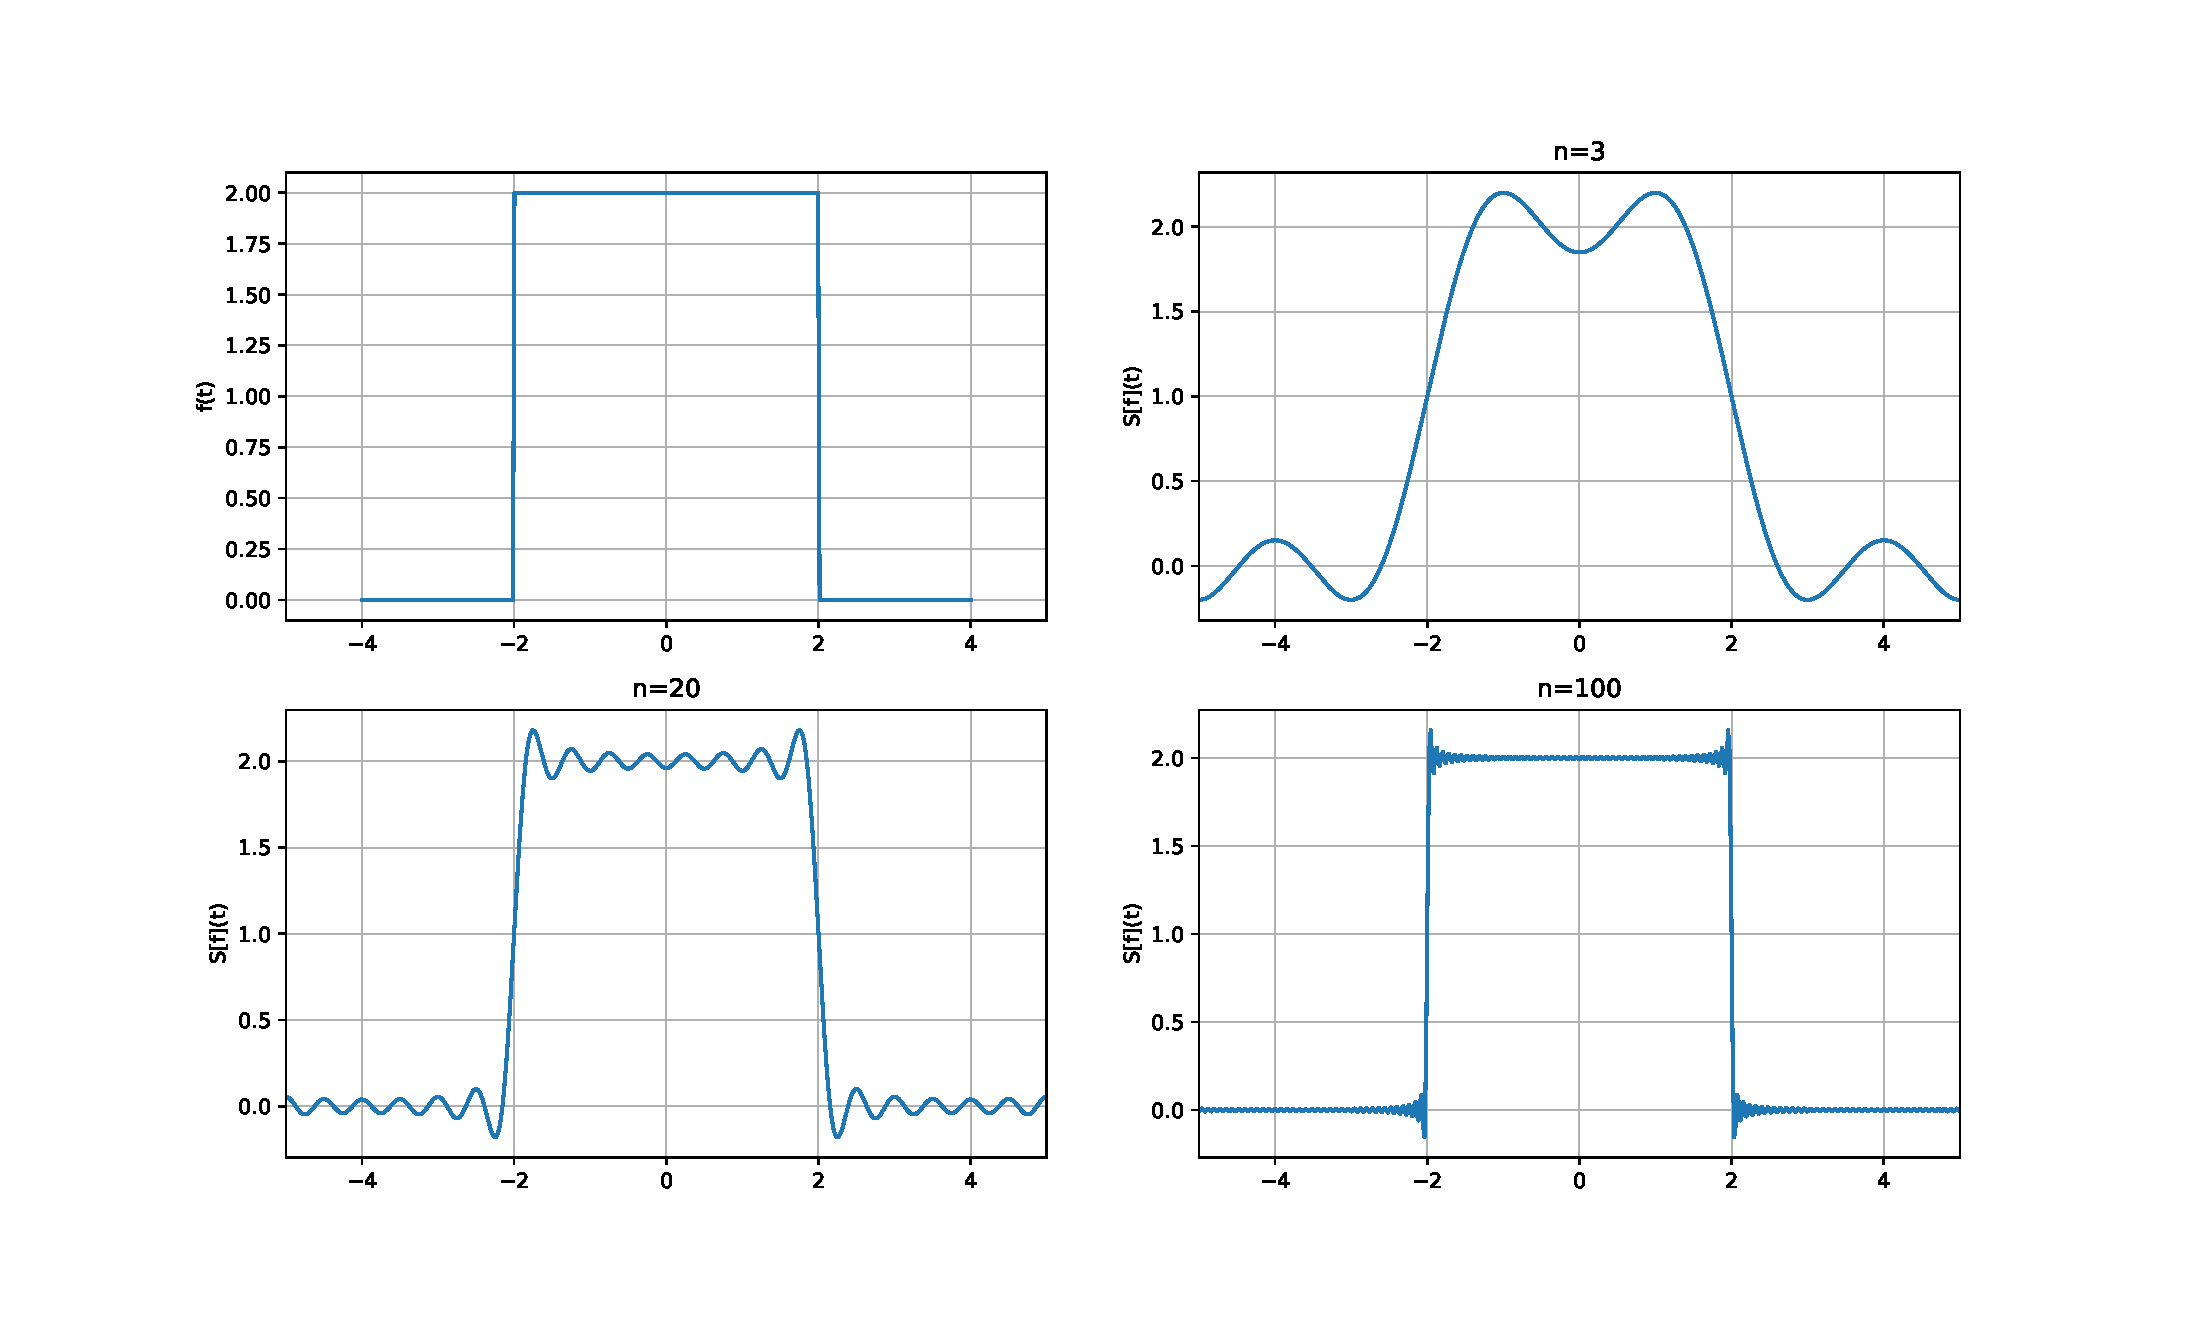
\includegraphics[width=\textwidth]{gibbs2.eps}
    \caption{吉布斯现象}
\end{figure*}

把图像画出来,可以发现随着逼近程度的增加(即\(n\)不断增大),部分和在间断点两侧的值总是会出现峰值无法减小的震荡(这个峰值又称为\uline{超调量}),超调量几乎与\(n\)无关,但是与跳跃的高度成正比. 设跳跃的高度为\(a\),随着\(n\)的增加,超调量的值近似为\(\beta a=0.0895a\),即大约\(9\%\).

用数学语言来描述,设被展开函数为\(f(x)\),其复数项傅里叶级数的部分和为\(S_N[f](x)\),即
\[ S_N[f](x) = \sum_{n=-N}^{N} c_ke^{in\omega x} = \sum_{n=-N}^{N}\int_T f(t)e^{-in\omega t}\trm{d}t e^{in\omega x} = \sum_{n=-N}^{N}\int_Tf(t)e^{in\omega(x-t)}\trm{d}t \]
根据控制收敛定理,此时有\(\lim \limits_{\substack{n \to \infty}}f_n(x)=f(x)\)
\begin{theorem}{吉布斯现象(Gibbs' phenomenon)}
    若\(f(x)\)的周期为\(T\),跳跃间断点为\(x_0\),两端值之差\(f(x_0^+)-f(x_0^-)=a\),则有
    \[\lim_{N \to \infty} S_N[f]\left(x_0+\frac{T}{2N}\right)=f(x_0^+)+\beta a\]
    \[\lim_{N \to \infty} S_N[f]\left(x_0-\frac{T}{2N}\right)=f(x_0^-)-\beta a\]
    其中\(\beta\)表示超调量相对于跳跃高度的比例,为
    \[\beta=\frac{1}{\pi}\int_{0}^{\pi}\frac{\sin(x)}{x}\trm{d}x-\frac{1}{2} \approx 0.08948987 \cdots\]
\end{theorem}
\textit{
    证明:设\(h(x)\)为\([0,T]\)上的连续函数,且导函数也连续,在\([0,T]\)内随机选择两点\(a,b(b>a)\),记\(b-a=L\),然后构造一个以\(T\)为周期的函数\(f(x)\)在\([0,T]\)内定义为
    \[f(x)=\left\{\begin{aligned} & h(x), & 0 < a \leq x < b < T \\ & 0, & \mbox{其他情况} \end{aligned}\right.\]
    这时\(f(x)\)就有了两个跳跃间断点\(x=a\)和\(x=b\),接下来仅证明
    \[\lim_{N\to \infty} S_N[f](a+\frac{T}{2N})=f(a^+)(1+\beta)\]
    \(f(a^-),f(b^+),f(b^-)\)的情况类似.
}

\vspace{1cm}

\textit{
    \(f(x)\)的复数形式的傅里叶级数的系数
    \[c_n = \frac{1}{T} \int_{0}^{T} f(t)e^{-in\omega t}\trm{d}t = \frac{1}{T} \int_{a}^{b}h(t)e^{-in\omega t}\trm{d}t\]
    整理\(S_N[f](x)\),把求和项全变成正的
    \[S_N[f](x) = c_0+\frac{1}{T}\sum_{n=1}^{N}\int_{a}^{b}h(t)\left(e^{in\omega(x-t)}+e^{-in\omega(x-t)}\right)\trm{d}t = c_0+\frac{2}{T}\sum_{n=1}^{N}\int_{a}^{b} h(t)\cos[n\omega(x-t)]\trm{d}t\]
    对其使用分部积分
    \begin{align*}
        & \int_{a}^{b}h(t)\cos[n\omega(x-t)]\trm{d}t \\
        &= \left.\left[\frac{-1}{n\omega}h(t)\sin[n\omega(x-t)]\right]\right|_{a}^{b}-\int_{a}^{b} h'(t)\left[\frac{-1}{n\omega}\sin[n\omega(x-t)]\trm{d}t\right] \\
        &= \frac{1}{n\omega}h(a)\sin[n\omega(x-a)] - \frac{1}{n\omega}h(b)\sin[n\omega(x-b)] + \frac{1}{n\omega}\int_{a}^{b}h'(t)\sin[n\omega(x-t)]\trm{d}t
    \end{align*}
    再代回原式
    \[S_N[f](x) = c_0+\frac{h(a)}{\pi}\sum_{n=1}^{N}\frac{\sin[n\omega(x-a)]}{n} - \frac{h(b)}{\pi}\sum_{n=1}^{N}\frac{\sin[n\omega(x-b)]}{n} + \frac{1}{\pi}\sum_{n=1}^{N}\frac{1}{n}\int_{a}^{b}h'(t)\sin\left[n\omega(x-t)\right]\trm{d}t\]
    于是
    \begin{align*}
        S_N[f]\left(a+\frac{T}{2n}\right) &= c_0 +\frac{h(a)}{\pi}{\color{red}\sum_{n=1}^{N}\frac{1}{n}\sin\left(\frac{n\pi}{N}\right)} 
        -\frac{h(b)}{\pi}{\color{blue}\sum_{n=1}^{N}\frac{1}{n}\sin\left(\frac{n\pi}{N}+n\omega L\right)} \\
        & \quad +\frac{1}{\pi}{\color{brown}\sum_{n=1}^{N}\frac{1}{n}\int_{a}^  {b}f'(t)\sin\left[\frac{n\pi}{N}+n\omega(t-a)\right]\trm{d}t} \\
        &= \frac{1}{T}\int_{a}^{b}h(t)\trm{d}t + \frac{h(a)}{\pi}{\color{red}I_1(N)}+ \frac{h(b)}{\pi}{\color{blue}I_2(N)} + \frac{1}{\pi}{\color{brown}I_3(N)}
    \end{align*}
    接下来分别讨论这三段,第一段恰好可以凑出黎曼和
    \begin{align*}
        {\color{red}I_1(\infty)} & = \lim_{N \to \infty}{\color{red}\sum_{n=1}^{n}\frac{1}{n}\sin\left(\frac{n\pi}{N}\right)} \\
        &=  \lim_{N \to \infty} \sum_{n=1}^{N}\frac{\pi}{N}\frac{\sin\left(\frac{n\pi}{N}\right)}{\frac{n\pi}{N}}  = \pi \lim_{N\to\infty} \sum_{n=1}^{N}\frac{1}{N}\trm{sinc}\left(\frac{n\pi}{N}\right)\\
        &= \pi\int_{0}^{1}\frac{\sin(\pi x)}{\pi x}\trm{d}x = \trm{Si}(\pi) = \pi\left(\frac{1}{2}+\beta\right)
    \end{align*}
    至于第二段,需要给出一个引理
}
\begin{lemma}{}
    \[\sum_{n=1}^{\infty}\frac{\sin(kn)}{n}=\frac{\pi-k}{2}\]
\end{lemma}
\textit{
    该引理的证明:构造\((0,\pi]\)上的函数
    \[f(x)=\left\{\begin{aligned} &\frac{\pi-x}{2}, &x \in [0,\pi] \\ &\frac{-\pi-x}{2}, & x \in (-\pi, 0) \end{aligned} \right. \]
    是奇函数,展成傅里叶级数之后只存在\(\sin\)项
    \[b_n = \frac{1}{\pi}\int_{-\pi}^{\pi}f(x)\sin(nx)\trm{d}x = \frac{2}{\pi}\int_{0}^{\pi}\frac{\pi-x}{2}\sin(nx)\trm{d}x=\frac{1}{n}\]
    因此在\([0,\pi]\)上\(\displaystyle{\frac{\pi-x}{2}=\sum_{n=1}^{\infty}\frac{\sin(nx)}{n}}\),引理证毕.
}

\textit{
    根据引理,有
    \begin{align*}
        {\color{blue}I_2(\infty)} 
        &= \lim_{N \to \infty}{\color{blue}\sum_{n=0}^{N}\frac{1}{n}\sin\left(\frac{n\pi}{N}-n\omega L \right)} 
        = \lim_{N \to \infty}{\color{blue}\sum_{n=0}^{N}\frac{1}{n}\sin \left[n\left(\frac{\pi}{N}-\omega L \right)\right]} \\
        & \sim \lim_{N \to \infty} \frac{\pi-\left(\frac{\pi}{N}-\omega L \right)}{2}
        = \pi\left(\frac{L}{T}-\frac{1}{2}\right)
    \end{align*}
    第三段也可以根据引理得到
    \begin{align*}
        {\color{brown}I_3(\infty)} &= \lim_{N \to \infty}{\color{brown}\sum_{n=1}^{N}\frac{1}{n}\int_{a}^{b}f'(t)\sin\left[\frac{n\pi}{N}+n\omega(t-a)\right]\trm{d}t} \\
        &= \lim_{N \to \infty} \int_{a}^{b}h'(t)\sum_{n=1}^{N}\frac{1}{n}\sin\left[\frac{n\pi}{N}+n\omega(t-a)\right]\trm{d}t \\
        \mbox{\textnormal{(根据引理)}} &= \pi \int_{a}^{b}h'(t)\left(\frac{t-a}{T}-\frac{1}{2}\right)\trm{d}t \\
        &= \frac{\pi}{T}\int_{a}^{b}h'(t)t\trm{d}t-\pi\left(\frac{a}{T}+\frac{1}{2}\right)\int_{a}^{b}h'(t)\trm{d}t \\
        \mbox{\textnormal{(分部积分)}} &= \frac{\pi}{T}\left[h(b)b-h(a)a-\int_{a}^{b}h(t)\trm{d}t\right]-\pi[h(b)-h(a)]\left(\frac{a}{T}+\frac{1}{2}\right)
    \end{align*}
    回代,得到
    \begin{align*}
        & \lim_{N \to \infty} S_N[f]\left(a+\frac{T}{2N}\right) \\
        &= \frac{1}{T}\int_{a}^{b}h(t)\trm{d}t+h(a)\left(\frac{1}{2}+\beta\right)-h(b)\left(\frac{L}{T}-\frac{1}{2}\right) \\
        & \quad +\frac{1}{T}\left[h(b)b-h(a)a-\int_{a}^{b}h(t)\trm{d}t\right] - [h(b)-h(a)]\left(\frac{a}{T}+\frac{1}{2}\right) \\
        &= h(a)\left(\frac{1}{2}+\beta-\frac{a}{T}+\frac{a}{T}+\frac{1}{2}\right) + h(b)\left(\frac{L}{T}-\frac{1}{2}+\frac{b}{T}-\frac{a}{T}+\frac{1}{2}\right) \\
        &= h(a)(1+\beta)
    \end{align*}
    这就定量求出了吉布斯现象的超调量为\(\beta=\dfrac{\trm{Si(\pi)}}{\pi}-\dfrac{1}{2} \approx 0.08948987 \cdots\).
}

\subsubsection{狄利克雷核}

狄利克雷核是一系列函数的统称,引入狄利克雷核可以更方便地讨论收敛性.

\begin{definition}{狄利克雷核}
    函数
    \[D_n(x) = \sum_{k=-n}^{n}e^{ikx}\]
    称为\(n\)阶\uline{狄利克雷核}(Dirichlet kernel).
\end{definition}

狄利克雷核具有如下性质:
\begin{itemize}
    \item [(1)] 狄利克雷核可以写成闭合表达式
    \[D_n(x)=\frac{\sin\left(\frac{2n+1}{2}x\right)}{\sin\left(\frac{1}{2}x\right)}\]
    \textit{
        证明:根据欧拉公式
        \[D_n(x) = \sum_{k=-n}^{n}e^{ikx} = 1+\sum_{k=1}^{n}(e^{ikx}+e^{-ikx}) = 1+2\sum_{k=1}^{n}\cos(nx)\]
        两边同乘\(\sin(x/2)\),用积化和差
        \begin{align*}
            \sin\left(\frac{x}{2}\right)D_n(x) &= \sin\left(\frac{x}{2}\right)+\sum_{k=1}^{n}2\sin\left(\frac{x}{2}\right)\cos(nx) \\
            &= \sin\left(\frac{x}{2}\right)+\sum_{k=1}^{n}\left[\sin\left(\frac{2n+1}{2}x\right)-\sin\left(\frac{2n-1}{2}x\right)\right] \\
            &= \cancel{\sin\frac{x}{2}}+\cancel{\sin\frac{3x}{2}}-\cancel{\sin\frac{x}{2}}+\cancel{\sin\frac{5x}{2}}-\cancel{\sin\frac{3x}{2}}+\cdots+\sin\frac{(2n+1)x}{2} \\
            &= \sin\frac{(2n+1)x}{2}
        \end{align*}
        因此\(\displaystyle{D_n(x)=\frac{\sin\left(\frac{2n+1}{2}x\right)}{\sin\left(\frac{1}{2}x\right)}}\)
    }
    \item [(2)] 傅里叶级数的部分和可以写成函数本身与\(n\)阶狄利克雷核的周期卷积
    \[S_n[f](x) = (f*D_n)(x)\]
\end{itemize}

\subsubsection{在原点处的间断点收敛性讨论}

\begin{definition}{利普希茨条件}
    若函数\(f(x)\)在某个邻域\(B(x_0,\delta)\)内满足
    \[|f(x)-f(x_0)| \leq C|x-x_0|^\alpha\]
    则称函数\(f(x)\)在\(x_0\)处满足\(\alpha\)阶\uline{利普希茨条件}(Lipschitz condition);
    \newline
    如果\(f(x)\)在定义域内处处满足利普希茨条件,则称\(f(x)\)满足\uline{一致的}(uniform)利普希茨条件;
    \newline
    如果将邻域\(B(x_0,\delta)\)改为单边邻域\([x_0,x_0+\delta)\),则称\(f(x)\)满足\uline{单边的}(unilateral)利普希茨条件.
\end{definition}

试想\(\alpha>1\),则有\(\displaystyle{\frac{|f(x)-f(x_0)|}{|x-x_0|} \leq C|x-x_0|^{\alpha-1}}\),再令\(x\to x_0\)即得到\(f'(x)=0\),则限制了\(f(x)\)必须为常值函数,这不是我们想要的结果,所以一般要求\(0<\alpha<1\). 接下来令函数\(f(x)\)在\(x_0\)的左右两侧都满足单边利普希茨条件.

接下来详细证明\(f(x)\)在\(x=0\)处出现跳跃间断点(函数在\(x=0\)处不连续但\(f(0^\pm)\)存在)时,\(S_{\infty}[f](0)\)会等于什么(剧透警告:会等于\(f(0^\pm)\)的算术平均).

\vspace{1cm}

\textit{
    根据狄利克雷核的两个性质:\(\displaystyle{S_N[f](x) = \frac{1}{2\pi}\int_{-\pi}^{\pi}f(x-t)D_N(t)\trm{d}t}\)和\(\displaystyle{\frac{1}{2\pi}\int_{-\pi}^{\pi}D_N(t)\trm{d}t=1}\),可以得到下面这个式子
}
\begin{align*}
    S_N[f](x)-f(x) &= \frac{1}{2\pi}\int_{-\pi}^{\pi}f(x-t)D_N(t)\trm{d}t - \frac{1}{2\pi}\int_{-\pi}^{\pi}f(x)D_N(t)\trm{d}t \\
    &= \frac{1}{2\pi}\int_{-\pi}^{\pi}[f(x-t)-f(x)]D_N(t)\trm{d}t 
\end{align*}
\textit{
    令\(\displaystyle{\overline{f}(x_0)=\frac{f(x_0^+)+f(x_0^-)}{2}}\),根据狄利克雷核的奇偶性将式子整理一下
}
\begin{align*}
    2\pi\left(S_N[f](x_0)-\overline{f}(x_0)\right) 
    &= \int_{-\pi}^{\pi}\left[f(x_0-t)-\frac{f(x_0+)}{2}-\frac{f(x_0^-)}{2}\right]D_N(t)\trm{d}t \\
    &= \left(\int_{-\pi}^{0}+\int_{0}^{\pi}\right)f(x_0-t)D_N(t)\trm{d}t-\left[\frac{f(x_0^+)}{2}+\frac{f(x_0^-)}{2}\right]\left(\int_{-\pi}^{0}+\int_{0}^{\pi}\right)D_N(t)\trm{d}t \\
    \mbox{(奇偶性)} &= \int_{0}^{\pi}[f(x_0-t)-f(x_0^-)]D_N(t)\trm{d}t+\int_{-\pi}^{0}[f(x_0-t)-f(x_0^+)]D_N(t)\trm{d}t \\
    &\quad + \cancel{\left[\frac{f(x_0^-)}{2}-\frac{f(x_0^+)}{2}\right]\int_{0}^{\pi}D_N(t)\trm{d}t} + \cancel{\left[\frac{f(x_0^+)}{2}-\frac{f(x_0^-)}{2}\right]\int_{-\pi}^{0}D_N(t)\trm{d}t} \\
    &= \int_{0}^{\pi}[f(x_0-t)-f(x_0^-)]D_N(t)\trm{d}t+\int_{-\pi}^{0}[f(x_0-t)-f(x_0^+)]D_N(t)\trm{d}t \\
    \mbox{(拆成4段)} &= \int_{0}^{\delta}[f(x_0-t)-f(x_0^-)]D_N(t)\trm{d}t + \int_{\delta}^{\pi}[f(x_0-t)-f(x_0^-)]D_N(t)\trm{d}t \\
    & \quad + \int_{-\pi}^{-\delta}[f(x_0-t)-f(x_0^+)]D_N(t)\trm{d}t + \int_{-\delta}^{0}[f(x_0-t)-f(x_0^+)]D_N(t)\trm{d}t \\
    &= I_1+I_2+I_3+I_4
\end{align*}
\textit{接下来就分别研究这四段,首先进一步整理\(I_3\),注意到}
\[D_N(t) = \frac{\sin[(N+\frac{1}{2})t]}{\sin\frac{t}{2}} = \frac{\sin(Nt)\cos(\frac{t}{2})+\cos(Nt)\sin(\frac{t}{2})}{\sin\frac{t}{2}} = \sin(Nt)\cot\frac{t}{2}+\cos(Nt)\]
所以将\(I_3\)拆成两部分
\begin{align*}
    I_3 &= \int_{-\pi}^{-\delta}[f(x_0-t)-f(x_0^+)]D_N(t)\trm{d}t \\
    &= \int_{-\pi}^{\delta}[f(x_0-t)-f(x_0^+)]\cot\frac{t}{2}\sin(Nt)\trm{d}t + \int_{-\pi}^{\delta}[f(x_0-t)-f(x_0^+)]\cos(Nt)\trm{d}t \\
    &= {\color{red}\int_{-\pi}^{\pi}}[f(x_0-t)-f(x_0^+)]\cot\frac{t}{2}\chi_{[-\pi,-\delta]}(t){\color{red}\sin(Nt)\trm{d}t} + {\color{red} \int_{-\pi}^{\pi}}[f(x_0-t)-f(x_0^+)]\chi_{[-\pi,-\delta]}(t){\color{red}\cos(Nt)\trm{d}t}
\end{align*}
\textit{其中\(\chi_S(x)\)是示性函数,定义为}
\[\chi_S(x) = \left\{\begin{aligned} & 1, & x \in S \\ & 0, &x \not\in S \end{aligned}\right.\]
\textit{
    一般地,将傅里叶系数分成实部和虚部两部分,即
    \[\int_{-\pi}^{\pi}f(t)e^{iNt}\trm{d}t = \int_{-\pi}^{\pi}f(t)\cos(Nt)\trm{d}t + i\int_{-\pi}^{\pi}f(t)\sin(Nt)\trm{d}t\]
    而根据黎曼-勒贝格引理,当\(N\to\infty\)时傅里叶系数趋于\(0\),其实部和虚部都要趋于\(0\),因此\(\displaystyle{\lim_{N\to\infty}I_3 \to 0}\),同理\(\displaystyle{\lim_{N\to\infty}I_2 \to 0}\).
    接下来讨论\(I_1\)和\(I_4\),首先对\(I_4\)放缩一下
}
\begin{align*}
    |I_4| &= \left|\int_{-\delta}^{0}[f(x_0-t)-f(x_0^+)]D_N(t)\trm{d}t\right| = \left|\int_{-\delta}^{0}\frac{f(x_0-t)-f(x_0^+)}{t}tD_N(t)\trm{d}t\right| \\
        &\leq \int_{-\delta}^{0}\left|\frac{f(x_0-t)-f(x_0^+)}{t}uD_N(t)\right|\trm{d}t
\end{align*}

\subsubsection{在任意处间断点的收敛性讨论}

TBD

跨越千山万水,经过了好几页的数学推导,我们终于得到了傅里叶级数收敛的定理.
\begin{theorem}{傅里叶级数收敛定理/狄利克雷定理}
    若函数\(f(x)\)的周期为\(T\),或仅在一个长度为\(T\)的区间上有定义,同时满足以下三个条件:
    \begin{itemize}
        \item [(1)] \(f(x)\)在一个周期区间上绝对可积,即\(\displaystyle{\int_{T} |f(x)|\trm{d}x < +\infty}\).
        \item [(2)] 在任意有界的区间内,\(f(x)\)只能存在有限个极值点.
        \item [(3)] 在任意有界的区间内,\(f(x)\)只能存在有限个第一类间断点.
    \end{itemize}
    以上三者称为\uline{狄利克雷条件}(Dirichlet conditions),此时该函数可以延拓成的\textbf{一致收敛的}傅里叶级数\(S_{\infty}[f](x)\),满足:
    \begin{itemize}
        \item [(1)] \(S_{\infty}[f](x)\)的定义域是\(\mathbb{R}\).
        \item [(2)] 若\(x\)是\(f(x)\)的连续点,那么\(S_{\infty}[f](x)=f(x)\).
        \item [(3)] 若\(x\)是\(f(x)\)的间断点,那么\(\displaystyle{S_{\infty}[f](x)=\lim_{h \to 0}\frac{f(x+h)+f(x-h)}{2}}\).
    \end{itemize}
\end{theorem}


\subsection{时域-频域的不确定性原理}
TBD
傅里叶带宽定理、Gabor极限,可以同海森堡不确定性原理相联系.

\subsection{单位冲激函数(狄拉克delta函数)}

讨论傅里叶变换怎能不提到它?毕竟它最初就随着傅里叶变换被首先提出来的(所以提出者不是狄拉克,但首先由狄拉克下了较为严格的定义). \uline{单位冲激函数}(unit impulse function)是一个非常特殊的函数,很难给出显式的定义,但其性质又决定了它具有广泛的用途.

\subsubsection{几种描述和近似}

最常见地,它由以下两个等式隐式地定义出来:
\[\left\{\begin{aligned} & \int_{-\infty}^{\infty}\delta(x)\trm{d}x=1 \\ & \forall x \neq 0: \delta(x)=0. \end{aligned}\right.\]
根据积分的几何意义容易发现,它在\(x=0\)处的值只能为正无穷大,这在黎曼积分的意义下是一种不可积的函数;即使\(x=0\)看成无穷间断点,那么黎曼积分为\(0\),而不可能是\(1\). 黎曼积分不允许它存在,这充分说明了\(\delta\)函数的特殊性.

至于这个函数是怎么被提出来的,最初傅里叶在《热分析理论》(\textit{Théorie analytique de la chaleur})一书中考虑了如下积分,把它用现在的形式写下来:
\[f(x) = \frac{1}{2\pi}\int_{-\infty}^{+\infty}\trm{d}\omega e^{i\omega x} \int_{-\infty}^{\infty}\trm{d}\alpha f(\alpha)e^{-i\omega x}\]
柯西把它改成了另一种更好看的形式
\[f(x) = \frac{1}{2\pi}\int_{-\infty}^{\infty}\left[\int_{-\infty}^{\infty}e^{i\omega(x-\alpha)}\trm{d}\omega\right]f(\alpha)\trm{d}\alpha\]
可以看出,反常积分\[\int_{-\infty}^{\infty}e^{i\omega(x-\alpha)}\trm{d}\omega\]被单独提了出来,起到了筛选的作用,乘上适当的系数,命名为一个函数,就是现在的\(\delta\)函数:
\[\delta(x-\alpha)=\frac{1}{2\pi}\int_{-\infty}^{\infty}e^{i\omega(x-\alpha)}\trm{d}\omega\]
把它代入傅里叶变换,得到
\[\mathcal{F}\left[\delta(x-\alpha)\right](\omega) = \int_{-\infty}^{\infty}\delta(x-\alpha)e^{-i\omega x}\trm{d}x = e^{-i\omega\alpha}\]
当\(\alpha=0\)时积分值为1,因此\(\delta\)函数的傅里叶变换为常函数\(\hat{f}(\omega)\equiv 1\).

\vspace{1cm}

尽管\(\delta\)函数的性质比较特殊,但可以利用某些“正常”的函数,通过调整某些参数,来逼近\(\delta\)函数. 严格地说,我们希望找到“正常”函数组成的序列\(\{f_n(x)\}_{n=1}^{\infty}\),满足以下几条类\(\delta\)函数的性质:
\begin{itemize}
    \item[(1)] 最值在\(x=0\)处取到:\[f_n(x)_{\trm{max}}=f_n(0)\]
    \item[(2)] 全域积分为1:\[\int_{-\infty}^{\infty}f_n(x)\trm{d}x=1\] 
    \item[(3)] 逼近性质:\[\lim_{n\to\infty}f_n(0)=+\infty\] 
\end{itemize}
随着\(n\)的增大,\(f_n(x)\)的形态就越来越接近\(\delta\)函数,以下列举几个例子:
\begin{itemize}
    \item [(1)] 采样函数
    \[f_n(x)=\frac{\sin(nx)}{\pi x}\]
    \item [(2)] 正态分布钟形曲线
    \[f_n(x)=\frac{1}{\sqrt{\pi n}}\exp\left(-\frac{x^2}{n}\right)\]
    \item [(3)] 泊松核
    \[f_n(x) = \frac{1}{\pi}\frac{n}{x^2+n^2}\]
    \item [(4)] 柯西主值(其实等价于采样函数)
    \[f_n(x) = \int_{-n}^{n}e^{i\omega x}\trm{d}\omega\]
\end{itemize}

\begin{figure*}[hbtp]
    \centering
    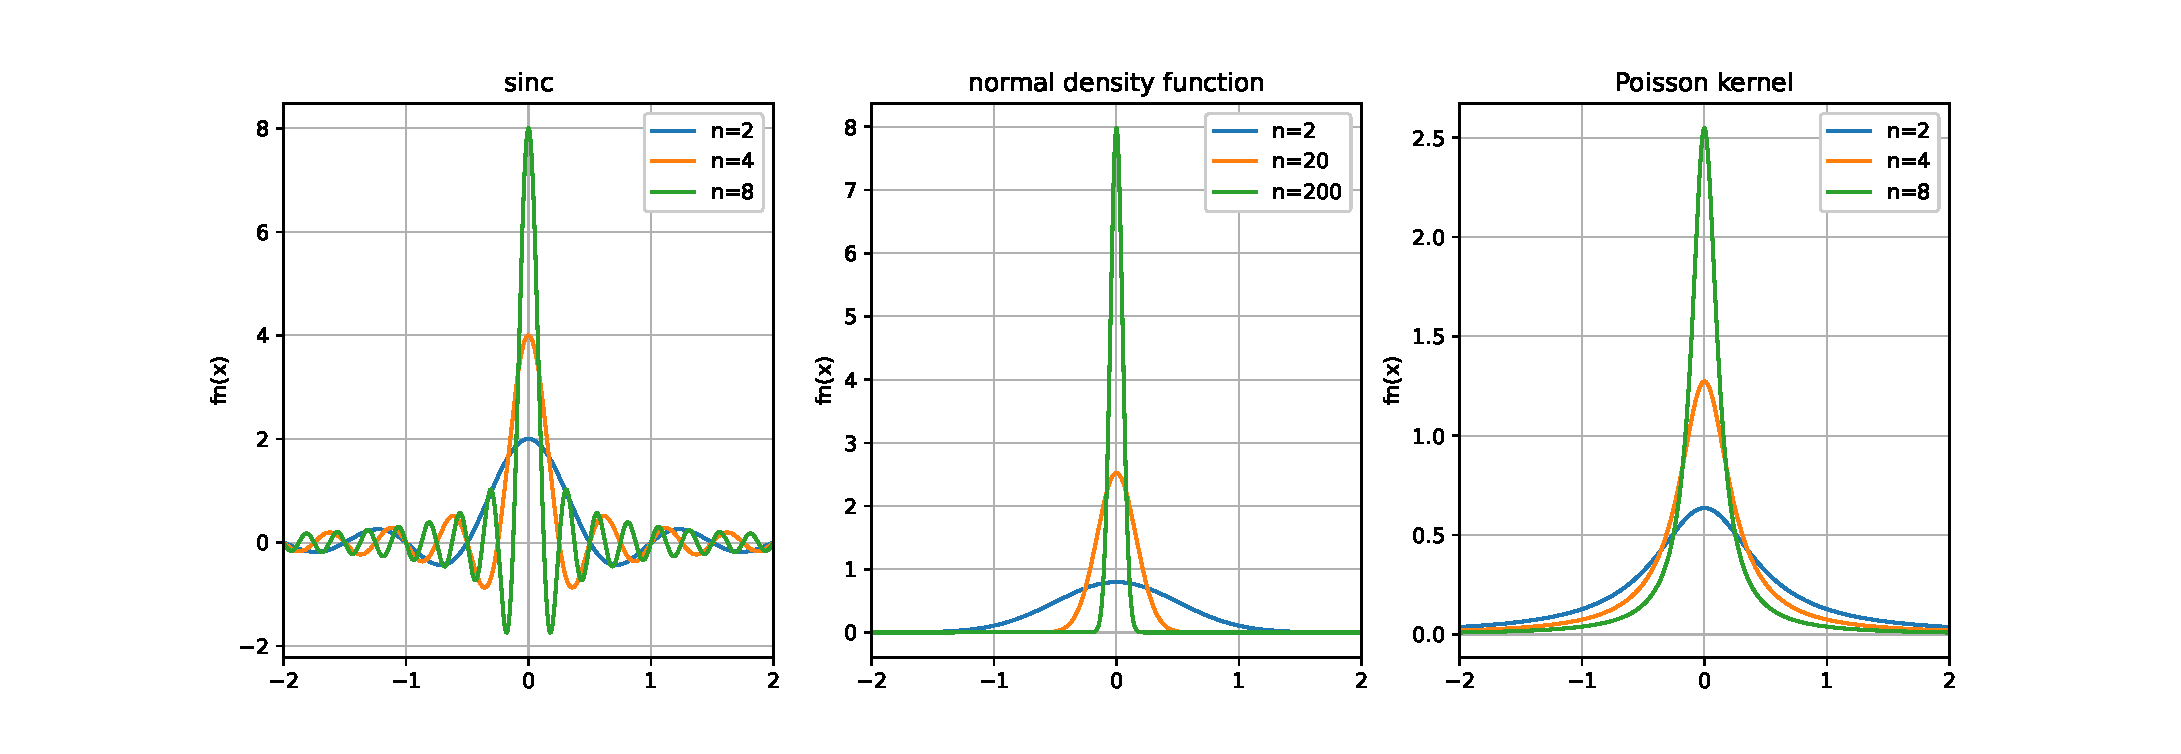
\includegraphics[width=\textwidth]{deltaapprox.eps}
    \caption{\(\delta\)函数的逼近}
\end{figure*}

\subsubsection{关于积分定义的问题}

以上提到,\(\delta\)函数是\(\displaystyle{f_n(x) = \frac{1}{2\pi}\int_{-n}^{n}e^{i\omega x}\trm{d}\omega}\)在\(n \to \infty\)时的形式极限,即可以说:
\[\delta(x) \sim \frac{1}{2\pi}\int_{-\infty}^{+\infty}e^{i\omega x}\trm{d}\omega\]
现在来仔细计算这个积分. 当\(x=0\)时,\(e^{i\omega x} \equiv 1\),因此积分值为正无穷,符合\(\delta\)函数的特征. 但当\(x \neq 0\)时,有
\[\int_{-\infty}^{+\infty}e^{i\omega x}\trm{d}\omega = \lim_{a \to +\infty} \int_{-a}^{+a}e^{i\omega x}\trm{d}\omega = \lim_{a \to +\infty}\left.\frac{1}{ix}e^{i\omega x}\right|_{-a}^{a} = \lim_{a \to +\infty}\frac{e^{iax}-e^{-iax}}{2ix} = \lim_{a \to +\infty}\frac{2}{x}\sin(ax)\]
这个极限是不存在的,因此利用积分直接定义\(\delta\)函数其实是有问题的,当然也有如下狡辩:
\begin{itemize}
    \item [\(\bullet\)] \textbf{狡辩1} 可改写以上极限,
    \[\lim_{a \to +\infty}\frac{2}{x}\sin(ax) = \lim_{a \to +\infty}2\pi \frac{\sin(ax)}{\pi x}\] 
    其中\(\displaystyle{\lim_{a \to +\infty}\frac{\sin(ax)}{\pi x} \sim \delta(x)}\),因此原极限收敛于\(2\pi\delta(x)\).
    \item[\(\bullet\)] \textbf{狡辩2} 可改写以上积分,
    \begin{align*}
        \int_{-\infty}^{+\infty}e^{i\omega x}\trm{d}\omega &= \lim_{\varepsilon \to 0}\int_{-\infty}^{+\infty}e^{i\omega x}e^{-\varepsilon\omega^2}\trm{d}\omega = \lim_{\varepsilon \to 0}\exp\left(-\frac{x^2}{4\varepsilon}\right)\int_{-\infty}^{+\infty}\exp\left[-\varepsilon\left(\omega-\frac{ix}{2\varepsilon}\right)^2\right]\trm{d}\omega \\
        &= \lim_{\varepsilon \to 0}\sqrt{\frac{\pi}{\varepsilon}}\exp\left(-\frac{x^2}{4\varepsilon}\right) \sim 2\pi \delta(x)
    \end{align*}
    其中最后一个等号来源于后面要介绍的高斯积分.
\end{itemize}

利用该积分等效于\(\delta\)函数是可行的,但是单独将其拿出来就不严谨了. 
% \(\delta(x)\)的积分称为单位阶跃函数,或者赫维赛德\(\varepsilon\)函数,即
% \[\varepsilon(x) = \int_{-\infty}^{x}\delta(x)\trm{d}x\]
% 它满足
% \[\varepsilon(x)=\left\{\begin{aligned} & 0, & x < 0 \\ & 1, & x > 0 \end{aligned}\right.\]
% \(\varepsilon(0)\)的值需要另外约定,一般为\(0\)或者\(1/2\).

\subsubsection{冲激函数的严格定义}

严格定义\(\delta\)函数是一件困难的事情,因为它需要较多的代数和拓扑的知识储备,这一节将把这些储备抖出一部分. 首先定义拓扑的概念.

\begin{itemize}
    \item[\(\bullet\)] \textbf{定义(拓扑)}
    \newline
    令集合\(\mathcal{T}\)为\(S\)的子集构成的集合,同时满足以下三个条件:
    \begin{itemize}
        \item [(1)] \(\emptyset \in \mathcal{T}, \quad S \in \mathcal{T}\)
        \item [(2)] 若\(x,y \in \mathcal{T}\),则\(x \cap y \in \mathcal{T}\)
        \item [(3)] 对于任意\(i \in I\),若\(x_i \in \mathcal{T}\),则\(\bigcup x_i \in \mathcal{T}\).
    \end{itemize}
    \(\mathcal{T}\)称为\(S\)的\uline{拓扑}(topology),\(\mathcal{T}\)中的元素称为\uline{开集}(open set),其补集称为\uline{闭集}(closed set),\(S\)连同拓扑\(\mathcal{T}\)称为\uline{拓扑空间}(topological space).
\end{itemize}

看起来很抽象,但只要考虑一个特例\(\mathbb{R}\),将开集类比为开区间,逐条讨论起来就直观多了. 

首先“形式上”有\((a,a)=\{x: a<x<a\}=\emptyset\),因此空集可以看做是一个开区间. \(\mathbb{R}\)可以表示为\((-\infty,+\infty)\),因此实数集本身也是一个开区间,第一条说的就是这两个特殊的对象是开集. 但需要注意的是,这两个家伙也是闭集.

有限个开区间的交集一定是开区间,但无限个开区间的交集可能是闭区间,比如\(\{(a-\frac{1}{n}, b+\frac{1}{n})\}_{n=1}^{\infty}\)这无穷个开区间的交集即为闭区间\([a,b]\),第二条说的就是有限个开集的交集也是开集. 不信你可以在\([a,b]\)之外任取一个数,例如\(b+\varepsilon\),总存在\(n\)使得\(b<b+\frac{1}{n}<b+\varepsilon\),因此这个\(b+\varepsilon\)就不属于这些集合的交集.

并集则不同,即使无限多个并集,无论是可数无限还是不可数无限,它们的并集的边界都是“开”的,例如并集\((1,2)\cup(3,4)\cup(5,6)\),尽管不连通,但它们的边界都是“开”的,都是小括号,因此这是一个开集,又例如区间\(\{(0,n)\}_{n=1}^{\infty}\),取了并集就是\((0,+\infty)\),也是个开集. 第三条把这些边界为“开”的区间纳入了开集的范围内.

由上所述,实数集以及全体边界为“开”的区间组成的集合组成了一个拓扑空间,但以实数集为基础的拓扑不止这一个,闭区间也可以包含在内,实数集的全体子集也可以组成一个拓扑,因此哪怕把范围限制在\(\mathbb{R}^n\)上,拓扑和开集也是一个非常抽象而广泛的概念,为了接下来的讨论更为方便,现在来明确\(\mathcal{T}\)的内容.

\begin{itemize}
    \item [\(\bullet\)] \textbf{定义(标准拓扑)}
    \newline
    拓扑空间\(\langle S, \mathcal{T} \rangle\)的结构如下:
    \begin{itemize}
        \item[(1)] 拓扑空间\(S=\mathbb{R}^n\),\(n\)为任意正整数.
        \item[(2)] 对于\(\mathbb{R}^n\)中的任意两个元素\(x=(x_1, x_2, \cdots, x_n)\)和\(y=(y_1,y_2,\cdots,y_n)\),度量规定为
        \[d(x,y)=\sqrt{(x_1-y_1)^2+(x_2-y_2)^2+\cdots+(x_n-y_n)^2}\]
        \item[(3)] 对于\(\mathbb{R}^n\)中的任意元素,开球定义为
        \[B_r(x_0) = \{x: d(x,x_0) < r\}\]
        \item[(4)] 对于任意\(\mathbb{R}\)的子集\(U\),若存在开球\(B_r(x_0) \subseteq U\),则\(U \in \mathcal{T}\).
    \end{itemize}
    由此得来的\(\langle S, \mathcal{T} \rangle\)称为\uline{标准拓扑}(standard topology).
\end{itemize}

标准拓扑中的开集限定得比刚才所说的“边界为‘开’的区间”更严格,除了空集和\(\mathbb{R}^n\)本身,对于\(\langle \mathbb{R}, \mathcal{T} \rangle\),开区间就是开集;对于\(\langle \mathbb{R}^2, \mathcal{T} \rangle\),单连通域去除其围线后的区域才能称为开集;对于\(\langle \mathbb{R}^3, \mathcal{T} \rangle\),封闭几何体去除其表面后的东西才能称为开集. 此时“开集”的概念已经非常直观了.

\begin{itemize}
    \item [\(\bullet\)] \textbf{定义(\(\mathbb{R}^n\)中的覆盖和紧集)}
    \newline
    在拓扑空间\(\langle \mathbb{R}^n,\mathcal{T} \rangle \)中,设\(S\)是集合,\(\{S_n\}_{n \in I}\)是一串开集,若\(S \subseteq \bigcup S_i\),则称\(\{S_n\}_{n \in I}\)是集合\(S\)的一个\uline{开覆盖}.
    \newline
    若闭集\(S\)的的每一个开覆盖都有有限子覆盖,则称\(S\)是\uline{紧集}(compact set).
\end{itemize}

覆盖的定义很形象,这一串开集就像一块块布去遮挡集合\(S\),每一块布料的“面积”可以有限也可以无限,每块布之间可以重叠也可以不重叠,如果能完全遮住,则这一堆布料就称为\(S)\)的开覆盖. 如果无论这些布料遮盖的方式如何,我都可以抽走某些布料,使得剩下有限块布料也能完全覆盖\(S\),那么这个\(S\)就被称为紧集. 可见,在\(\mathbb{R}^n\)中,紧集同有界闭集等价,因为如果集合是无界的,而每块布料都是“有限大”的,那么就不可能使用有限块布料覆盖该集合.

\begin{itemize}
    \item [\(\bullet\)] \textbf{定义(连续映射)}
    \newline
    设有两个拓扑空间\(\langle X, \mathcal{T}_1 \rangle\)和\(\langle Y, \mathcal{T}_2 \rangle\),以及映射\(f:X \to Y\),若对于任意\(V \in \mathcal{T}_2\),其原象
    \[\{x: f(x) \in V\} \in \mathcal{T}_1\]
    则称该映射\(f\)在拓扑意义上是\uline{连续的}(continuous).
    \item [\(\bullet\)] \textbf{定义(标准拓扑上的连续映射)}
    \newline
    设映射\(f:\mathbb{R}^m \to \mathbb{R}^n\),若对于任意开集\(U \subseteq \mathbb{R}^n\),若其原象\(f^{-1}(U)\)也是开集,则称该映射\(f\)在拓扑意义上是\uline{连续的}(continuous).
\end{itemize}

其实标准拓扑上的连续和“一致连续”这两个概念是等价的,证明略. 如果一个映射建立在向量拓扑空间中,而且对于该向量空间是线性的,对于该拓扑空间是连续的,则称该映射为“\textbf{连续线性映射}”. 

\begin{itemize}
    \item [\(\bullet\)] \textbf{定义(对偶空间和weak*拓扑)}
    \newline
    若\(\langle S ,\mathcal{T} \rangle\)是向量拓扑空间,则所有\(S \to \mathbb{R}\)的连续线性映射组成的集合称为\(S\)的\uline{对偶空间}(dual space),记作\(X^*\)
    \newline
    在\(X^*\)上建立拓扑,并定义映射\(f:X^* \to \mathbb{R}\),使得\(f\)是连续函数的包含开集最少的拓扑称为\(X^*\)的waek*拓扑.
\end{itemize}

weak*拓扑的定义有点抽象. 

\vspace{1cm}

基础知识已经铺好,接下来开始正式定义\(\delta\)函数. 由于\(\delta\)函数在\(\mathbb{R}^n\)上起作用,所以只用考虑其上的拓扑结构和函数空间.

\begin{itemize}
    \item [\(\bullet\)] \textbf{定义(函数的极限)}
    \newline
    将\(\mathbb{R}^n\)上全体具有紧致支撑集的任意次可微函数的集合记作\(C_c^{\infty}\left(\mathbb{R}^n\right)\),对于其中的函数序列\(\{\phi\}_{n=1}^{\infty}\),若存在\(\phi \in C_c^{\infty}\left(\mathbb{R}^n\right)\),使得
    \begin{itemize}
        \item [(1)] 存在紧致集\(K\),使得\(\phi_n\)的支撑集都是\(K\)的子集.
        \item [(2)] 随着\(n\)的增加,\(\phi_n\)以及它们的任意阶导数均收敛于\(\phi\)及其对应阶导数.
    \end{itemize}
    则称函数序列\(\{\phi_n\}_{n=1}^{\infty}\)收敛于\(\phi\),记作\(\displaystyle{\lim_{n \to \infty}\phi_n=\phi}\). 并规定\(C_c^{\infty}\left(\mathbb{R}^n\right)\)上的拓扑结构为满足此收敛方式且开集最少的拓扑.
\end{itemize}

\begin{itemize}
    \item [\(\bullet\)] \textbf{定义(\(\mathbb{R}^n\)中的支撑集)}
    \newline
    对于函数\(f:\mathbb{R}^n \to \mathbb{R}\),使得\(f(x) \neq 0\)的全体\(x\)的集合称为该函数的\uline{支撑集}(support set).
\end{itemize}

\subsection{采样和插值}

\subsubsection{采样定理}

采样定理是从连续到离散迈出的第一步,这个定理告诉我们,只要\(f(t)\)存在最高频率,那么可以等间距地记录\(f(t)\)的值,这些记录下来的离散的值可以完全确定连续的\(f(t)\).
\textit{
\newline
(以下推导过程是香农的原始思路)
\newline
假设\(f(t)\)的最高角频率是\(\omega_H\),意思是当\(\omega > \omega_H\)时,均有\(\hat{f}(\omega)=0\)(不一定无定义),那么在傅里叶逆变换时可以使用\(\omega_H\)来代替其积分上下界,即
\[f(t) = \mathcal{F}^{-1}[\hat{f}(\omega)](t) = \frac{1}{2\pi}\int_{-\infty}^{\infty}\hat{f}(\omega)e^{i\omega t}\trm{d}\omega = \frac{1}{2\pi}\int_{-\omega_H}^{\omega_H}\hat{f}(\omega)e^{i\omega t}\trm{d}\omega\]
若令\(B=2\omega_H\)表示双边带宽,则
\[\frac{2\pi}{B}f\left(-\frac{2\pi k}{B}\right) = \frac{1}{B}\int_{-B/2}^{B/2}\hat{f}(\omega)e^{\frac{i2\pi k\omega}{B}}\trm{d}\omega\]
将\(\hat{f}(\omega)\)延拓成复数项形式的傅里叶级数(周期自然是\(B\),另外这里\(\omega\)是哑变量,所以在展开式中直接写成\(2\pi/B\)),接着可以发现系数\(c_k\)能被换掉
\[ \hat{\tilde{f}}(\omega) = \sum_{k=-\infty}^{+\infty}{\color{red} c_k}e^{\frac{i2\pi k\omega}{B}} 
= \sum_{k=-\infty}^{+\infty} {\color{red} \left[\frac{1}{B} \int_{B}\hat{f}(\omega)e^{-\frac{i2\pi k\omega}{B}}\trm{d}\omega\right]}e^{\frac{i2\pi k\omega}{B}} 
= \sum_{k=-\infty}^{+\infty} {\color{red} \frac{2\pi}{B}f\left(-\frac{2\pi k}{B}\right)}e^{\frac{i2\pi k\omega}{B}}\]
仔细思考这个等式的含义,左边是\(f(t)\)的频谱函数,它经过反傅里叶变换即可得到完整的\(f(t)\),右边是个无穷级数,参与到该无穷级数运算的有关于\(f(t)\)的东西只有\(f(0), f(\pm 2\pi/\omega_B), f(\pm 4\pi/\omega_B), f(\pm 6\pi/\omega_B), \cdots\)这些离散的值. 这就意味着,只要知道了这些采样值,就可以知道\(f(t)\)每一点的值,而且是精确值.
\newline
在给出最终定理之前,再把式子整理一下. 考虑到\(B\)表示角频率(的差值),那么\(\displaystyle{\frac{2\pi}{B}}\)就具有了时间间隔的含义. 如果令\(\displaystyle{T_s=\frac{2\pi}{B}}\),并设\(\displaystyle{f[n]=f(nT_s)}\),再做个简单换元,就得到了时域采样定理.
}

\begin{theorem}{奈奎斯特-香农采样定理(Nyquist-Shannon sampling theorem)/低通采样定理}
    如果一个函数\(f(t)\)的角频率不超过\(\omega_H\),则\(f(t)\)可以被一系列间距为\(T_s=\dfrac{\pi}{\omega_H}\)的采样点确定. 此时\(f(t)\)的双边频带宽度\(B=2\omega_H\)也称为\uline{奈奎斯特抽样率}(Nyquist sampling rate),\(T_s\)称为\uline{奈奎斯特抽样间隔}(Nyquist sampling interval). 更进一步地,该函数对应的频域表达式为
    \[\hat{f}(\omega) = T_s \sum_{n=-\infty}^{\infty}f[n]e^{-iT_sn\omega}\]
\end{theorem}

换个角度想,为什么离散的采样值能

对偶地,有频域上的函数也有采样定理
\begin{corollary}{频域采样定理}
    如果时域函数\(f(t)\)仅在长度为\(T\)的区间内有定义,记\(\omega_0=\dfrac{2\pi}{T}\)为频域采样间隔,\(\hat{f}[n]=\hat{f}(n\omega_0)\)为频域采样序列,则根据这个序列可确定延拓出完整的时域函数
    \[\tilde{f}(t)=\frac{1}{T}\sum_{n=-\infty}^{+\infty}\hat{f}[n]e^{in\omega_0t}\]
    其中\(\tilde{f}(t)\)是\(f(t)\)的以\(T\)为周期的延拓.
\end{corollary}

接下来这条推论非常重要,它非常宏观地刻画了时域和频域的对偶性:时域和频域只要有一个域是离散的,那么另一个域就是连续且周期的的,反之成立. 这同时也否定了后面出现的离散傅里叶变换精确刻画原函数的可能性.

\begin{corollary}{周期性对偶}
    以\(T_s\)为采样间隔的序列所对应的频域函数具有周期\(\dfrac{2\pi}{T_s}\),以\(\omega_0\)为频域采样间隔的序列对应的时域函数具有周期\(\dfrac{2\pi}{\omega_0}\).
\end{corollary}
\textit{
    证明:直接代入即可
    \begin{align*}
        \hat{f}\left(\omega+\frac{2\pi}{T_s}\right) &= T_s \sum_{n=-\infty}^{\infty}f[n]\exp\left(-iT_sn(\omega+\frac{2\pi}{T_s})\right) = T_s \sum_{n=-\infty}^{\infty}f[n]\exp\left(-iT_sn\omega+i2n\pi\right) \\
        &= T_s \sum_{n=-\infty}^{\infty}f[n]\exp(-iT_sn\omega) = \hat{f}(\omega)
    \end{align*}
    频域的证明类似.
}

\subsubsection{插值公式:从采样点恢复原信号}

采样定理好是好,但想从采样点还原完整的\(f(t)\),要先计算一波无穷级数,然后再反傅里叶变换才行. 为何不现在就完成这个过程呢?
上式两边同时求傅里叶反变换,得到
\[f(t) = \frac{1}{2\pi}\int_{-\infty}^{\infty}\hat{f}(\omega)e^{i\omega t}\trm{d}\omega 
= \frac{1}{2\pi}\int_{-\omega_H}^{\omega_H}\hat{f}(\omega)e^{i\omega t}\trm{d}\omega 
= \int_{-\infty}^{\infty}\sum_{k=-\infty}^{+\infty} \frac{1}{\omega_B}f\left(-\frac{2\pi k}{\omega_B}\right)e^{\frac{i2\pi k\omega}{\omega_B} + i\omega t}\trm{d}\omega\]
根据控制收敛定理\footnote{\(\mathbb{C}\)上的控制收敛定理(dominated convergence theorem):设\(\{f_n(x)\}_{n=0}^{\infty}\)是一系列可测的且逐点收敛于\(f(x)\)的函数,若存在实函数\(g(x)\)使得任意\(n\)均有\(|f_n(x)|<g(x)\),则有\[\lim_{n \to \infty}\int f_n(x)\trm{d}x = \int f(x)\trm{d}x\]},交换积分与求和的顺序,同时提出与被积变量无关的部分
\[f(t) = \frac{1}{\omega_B}\sum_{k=-\infty}^{\infty}f\left(\frac{-2k\pi}{\omega_B}\right){\color{blue}\int_{-\omega_H}^{\omega_H}e^{\frac{i2\pi k\omega}{\omega_B} + i\omega t}\trm{d}\omega}\]
现在来看其中的积分项,恰好可以化成\(\trm{sinc}(x)\)的形式
\begin{align*}
    {\color{blue}\int_{-\omega_H}^{\omega_H}e^{\frac{i2\pi k\omega}{\omega_B} + i\omega t}\trm{d}\omega} 
    &= \int_{-\omega_H}^{\omega_H}\exp{\frac{i\omega(2k\pi+\omega_Bt)}{\omega_B}}\trm{d}\omega
    = \left.\frac{\omega_B}{i(2k\pi+\omega_Bt)}\exp{\frac{i\omega(2k\pi+\omega_Bt)}{\omega_B}}\right|_{-\omega_H}^{\omega_H} \\
    &= \omega_B\cdot\frac{\exp\left(i\frac{2k\pi+\omega_Bt}{2}\right) - \exp\left(-i\frac{2k\pi+\omega_Bt}{2}\right)}{\frac{2k\pi+\omega_Bt}{2}\cdot 2i} = \omega_B\trm{sinc}(k\pi+\omega_Ht)
\end{align*}
将其带回上式,就是采样定理的副产品:
\begin{theorem}{惠特克-香农插值公式(Whittaker-Shannon interpolation formula)}
    如果一个函数\(f(t)\)的角频率不超过\(\omega_H\),令\(T_s=\dfrac{\pi}{\omega_H}\)为奈奎斯特采样间隔,再令\(f[n]=f(nT_s)\)作为采样序列,则
    \[f(t) = \sum_{k=-\infty}^{\infty}f[n]\trm{sinc}\left(\omega_H(t-nT_s)\right)\]
\end{theorem}
之所以称为插值公式,连续函数\(f(t)\)可以看做\(f[n]\)的延拓,因为当\(T_s=1\)时,有\(f(n)=f[n]\).

\subsubsection{离散时间傅里叶变换}

采样定理说明了,完整的频域表达式可以由时域上间隔为\(T_s\)的采样点确定. 采样点组成的序列相当于取值限定在\(nT_s, n\in \mathbb{Z}\)的函数,而数列本身是取值限定在整数的函数. 若令\(T_s=1\),那么采样点序列也就成了数列. 这告诉我们,不仅是连续函数,数列也可以做傅里叶变换,为了有别于连续函数的傅里叶变换,时域采样序列的傅里叶变换称为“离散时间傅里叶变换”.

\begin{definition}{离散时间傅里叶变换}
    令\(\{f[n]\}_{n=-\infty}^{+\infty}\)为双边无限长的数列,且绝对可和,则
    \[\hat{f}(\omega)=\mathcal{F}\left[f[n]\right](\omega):=\sum_{n=-\infty}^{+\infty}f[n]e^{in\omega}\]
    称为该数列的\uline{离散时间傅里叶变换}(discrete-time Fourier transformation, DTFT),其逆变换为
    \[f[n]=\mathcal{F}^{-1}\left[\hat{f}(\omega)\right][n]:=\int_{-\pi}^{\pi}\hat{f}(\omega)e^{in\omega}\trm{d}\omega\] 
\end{definition}

\subsection{离散傅里叶变换}

众所周知,随机的连续函数承载无限的信息,无法用有限个字符描述出来. 哪怕经过采样定理的优化,时域和频域总有一个域是连续的,另一个虽然是离散的,但也是无限长且没有周期性的,仍然不能存储. 但假如给离散序列取一个有限长但长度很大的子序列,并抛弃其他部分,然后让这个子序列周期循环形成新的无限长序列,就可以在一定程度上模拟原来的无限长序列,同时还能保证在另一个域也是周期且离散的. 在周期且离散的序列之间做的时域-频域变换,就是离散傅里叶变换.

\begin{definition}{离散傅里叶变换}
    对于任意一个有限长序列\(\{f[n]\}_{n=0}^{N}\),定义
    \[\hat{f}[k]=\mathcal{F}[f[n]][k] = \sum_{n=0}^{N-1}f[n]\exp\left(-i\frac{2\pi kn}{N}\right), \qquad 0 \geq k \geq N-1\]
    称为序列\(f[n]\)的\uline{离散傅里叶变换}(discrete Fourier transform, DFT),其逆变换为
    \[f[n] = \mathcal{F}^{-1}\left[\hat{f}[k]\right][n] = \frac{1}{N}\sum_{k=0}^{N-1}\hat{f}[k]\exp\left(i\frac{2\pi kn}{N}\right), \qquad 0 \geq n \geq N-1\]
    其中记\(W_{N}=\exp\left(\dfrac{-2\pi i}{N}\right)\),称为\uline{旋转因子}.
\end{definition}

其中旋转因子\(W_{N}\),形象地理解,就是\(N\)个单位向量按角度平分了单位圆,以与实轴共线的单位向量为第\(0\)个,\(W_N^k\)就是顺时针数的第\(k\)个单位向量. \(W_N\)很大程度上决定了离散傅里叶变换的性质以及快速算法的可能性,接下来讨论它的性质,其中出现的变量\(k,n,N\)等默认为整数.
\begin{itemize}
    \item [(1)] 中心对称性:\(\overline{W_N^n}=W_N^{N-n}\).
    \item [(2)] 周期性:\(W_N^n=W_N^{n+N}\).
    \item [(3)] 可约性:\(W_N^n=W_{kN}^{kn}\).
    \item [(4)] 正交性:\(\displaystyle{\sum_{k=0}^{N-1}W_N^{kn}=\left\{\begin{aligned} &N,&k|N \\ &0,&k\not | N\end{aligned}\right.}\)
    \newline
    \textit{
        证明:从几何的角度,当\(k|N\)时,\(W_N^{kn}\equiv 1\),此时的求和即为\(N\times 1=N\),当\(k\not|N\)时,就套入等比数列求和公式:
        \[\sum_{k=0}^{N-1}W_N^{kn}=\sum_{k=0}^{N-1}\exp\left(\frac{-2\pi kni}{N}\right)=\frac{1-\exp\left(\frac{-2\pi \cancel{N} ni}{\cancel N}\right)}{1-\exp\left(\frac{-2\pi ni}{N}\right)}=0\]
    }
\end{itemize}

因此离散傅里叶变换有以下性质,记\(\hat{f}[k]=\mathcal{F}[f[n]][k]\)
\begin{itemize}
    \item [(1)] 线性
    \[\mathcal{F}[f_1[n]+f_2[n]][k]=\hat{f}_1[k]+\hat{f}_2[k]\]
    \textit{
        证明略.
    }
    \item [(2)] 可用正变换计算逆变换
    \[\mathcal{F}^{-1}\left[\hat{f}[k]\right][n] = \frac{1}{N}\overline{\mathcal{F}\left[\overline{\hat{f}[k]}\right][n]}\]
    \item [(3)] 时域-频域对偶性质
    \[\frac{1}{N}\mathcal{F}\left[\hat{f}[n]\right][k]=f[-k]\]
    \item [(4)] 取相反数
    \[\mathcal{F}[f[-n]][k]=\hat{f}[-k]\]
    \item [(5)] 域的求和
    \[\sum_{n=0}^{N-1}f[n]=\hat{f}[0]\]
    \[\sum_{k=0}^{N-1}\hat{f}[k]=Nf[0]\]
    \item [(6)] 序列加长
    在\(f[n]\)末端添加若干个\(0\)使其长度增加到\(rN\),即令
    \[g[n]=\left\{\begin{aligned}& f[n], & 0 \geq n \geq N-1 \\ & 0, N \geq n \geq rN-1 \end{aligned}\right.\]
    则
    \[\mathcal{F}[g[n]]=\hat{f}\left[\frac{k}{r}\right]\]
    \item [(7)] 圆周移位定理
    \[\mathcal{F}\left[\tilde{f}[n+m]\right]=W_N^{-km}\hat{\tilde{f}}[k]\]
    \item [(8)] 圆周卷积定理
    \item [(9)] 圆周相关定理
    \item [(10)] 帕斯瓦尔定理
    \item [(11)] 圆周对称性
    \newline
    这一条性质内容非常丰富,首先讨论序列的共轭对称分解:
    \begin{align*}
        f[n] & =\frac{1}{2}\left(2f[n]\right)=\frac{1}{2}\left(2f[n]+\overline{f[n]}-\overline{f[n]}\right) \\
        &= {\color{red}\frac{1}{2}\left(f[n]+\overline{f[-n]}\right)}+{\color{blue}\frac{1}{2}\left(f[n]-\overline{f[-n]}\right)}
    \end{align*}
    其中红色的部分取共轭之后仍然等于它本身(称为共轭对称性),蓝色的部分取共轭之后等于它的相反数(称为共轭反对称性),于是定义
    \begin{definition}{序列的共轭对称分解}
        对于任意一个序列\(f[n]\)均有\(f[n]=f_e[n]+f_o[n]\),其中
        \[f_e[n]=\frac{1}{2}\left(f[n]+\overline{f[-n]}\right)\]
        称为\(f[n]\)的\uline{共轭对称分量},
        \[f_o[n]=\frac{1}{2}\left(f[n]-\overline{f[-n]}\right)\]
        称为\(f[n]\)的\uline{共轭反对称分量}.
    \end{definition}
\end{itemize}

\subsection{快速(离散)傅里叶变换}
\subsubsection{基2-FFT算法}
TBD
\subsubsection{基4-FFT算法}
TBD
\subsubsection{库利-图基算法}
TBD
\subsubsection{Chirp-Z}
TBD

\subsection{拉普拉斯变换:给傅里叶变换打补丁}
TBD

\subsection{Z变换:给离散傅里叶变换打补丁}
TBD

\subsection{设计低通滤波器}
TBD

\end{document}